\documentclass[10pt,letterpaper]{article} % Font sizes smaller than 10pt are ignored here. Use scaled= in helvet.
%DIF LATEXDIFF DIFFERENCE FILE
%DIF DEL old.tex               Fri Oct 18 12:56:44 2024
%DIF ADD interop-mapping.tex   Fri Oct 18 13:10:59 2024
%DIF 2a2-5
 %DIF > 
% latexdiff old.tex interop-mapping.tex > diff.tex %DIF > 
% latexmk -pdf diff  %DIF > 
 %DIF > 
%DIF -------
% Some useful packages for including images, colored font, etc.
\usepackage{url}
%\usepackage[yyyymmdd,hhmmss]{datetime}
%\renewcommand{\dateseparator}{-}
\usepackage{pdfsync}
\usepackage{enumitem}
\usepackage{amsmath}
\usepackage{amssymb}
\usepackage{outline}
%\usepackage{dsfont} % pendant
\usepackage{comment}
\usepackage{lmodern}
\usepackage{cite}
\usepackage{float}
\usepackage{appendix}
\usepackage{fancyvrb}
%\usepackage{hyperref} % for href
\usepackage{textcomp} % has bullet, copyright symbols, etc.
\usepackage[skip=5pt plus1pt, indent=20pt]{parskip} % space between paragraphs

%\usepackage{inconsolata} % I can't find it on Pendant distribution. https://tex.stackexchange.com/questions/50810/good-monospace-font-for-code-in-latex    % pendant
% Currently I can't download inconsolate. Try later: https://ctan.org/tex-archive/fonts/inconsolata/?lang=en
% 2023-07-17 Ubuntu apparently doesn't have a full texlive distribution. I was
\usepackage{courier}    % Alternative monospace. Inconsolata is a bit rougher, but distinguishes ( from { better.  % pendant (uncomment)

\usepackage{listings,xcolor} % See https://en.wikibooks.org/wiki/LaTeX/Source_Code_Listings about minted rather than this.

\usepackage{graphicx}
\graphicspath{{./figures/}}
\graphicspath{{figures/}}

\usepackage[scaled=0.95]{helvet} % Sans serif font. https://mirror.las.iastate.edu/tex-archive/macros/latex/required/psnfss/psnfss2e.pdf
\renewcommand{\familydefault}{\sfdefault}

\bibliographystyle{unsrt}
\usepackage{fancyhdr}
\fancyhf{}
%\fancyhead[C]{\today\ DRAFT page \thepage}
\fancyhead[C]{page \thepage}
\pagestyle{fancy}

% This is only useful for courier; not needed for inconsolata.
%\newcommand{\stt}[1]{\begin{footnotesize}\texttt{#1}\end{footnotesize}}
\newcommand{\stt}[1]{\texttt{#1}} % I use this on Mint5.
\newcommand{\bdef}[1]{\textbf{\textit{#1}}}

\usepackage{makecell}      % cells in tables to handle multiline content (see Ch5)
\usepackage{hhline}        % more stuff for tables

\usepackage{geometry} % https://www.overleaf.com/learn/latex/Page_size_and_margins#Paper_size.2C_orientation_and_margins
 \geometry{
%  a4paper,
%  total={170mm,257mm},
   left=23mm,
   right=23mm,
   top=20mm,
   bottom=20mm
 }

 % ^^3f is a question mark (UTF-8)

% Begin JavaScript listinglst --------------------------------

\usepackage{color} %use color
\definecolor{mygreen}{rgb}{0,0.6,0}
\definecolor{myred}{rgb}{0.8,0.2,0.2}
\definecolor{mygray}{rgb}{0.5,0.5,0.5}
\definecolor{mymauve}{rgb}{0.58,0,0.82}

%Customize a bit the look
\lstset{ %
backgroundcolor=\color{white},   % choose the background color; you must add \usepackage{color} or \usepackage{xcolor}
basicstyle=\footnotesize,        % the size of the fonts that are used for the code
breakatwhitespace=false,         % sets if automatic breaks should only happen at whitespace
breaklines=true,                 % sets automatic line breaking
captionpos=b,                    % sets the caption-position to bottom
commentstyle=\color{mygreen},    % comment style
deletekeywords={...},            % if you want to delete keywords from the given language
escapeinside={\%*}{*)},          % if you want to add LaTeX within your code
extendedchars=true,              % lets you use non-ASCII characters; for 8-bits encodings only, does not work with UTF-8
%pod frame=single,               % adds a frame around the code
keepspaces=true,                 % keeps spaces in text, useful for keeping indentation of code (possibly needs columns=flexible)
keywordstyle=\color{blue},       % keyword style
%language=JavaScript,            % the default language of the code  CANNOT BE SET.
morekeywords={*,...},            % if you want to add more keywords to the set
numbers=left,                    % where to put the line-numbers; possible values are (none, left, right)
numbersep=5pt,                   % how far the line-numbers are from the code
numberstyle=\tiny\color{mygray}, % the style that is used for the line-numbers
rulecolor=\color{black},         % if not set, the frame-color may be changed on line-breaks within not-black text (e.g. comments (green here))
showspaces=false,                % show spaces everywhere adding particular underscores; it overrides 'showstringspaces'
showstringspaces=false,          % underline spaces within strings only
showtabs=false,                  % show tabs within strings adding particular underscores
stepnumber=1,                    % the step between two line-numbers. If it's 1, each line will be numbered
stringstyle=\color{mymauve},     % string literal style
tabsize=2,                       % sets default tabsize to 2 spaces
title=\lstname                   % show the filename of files included with \lstinputlisting; also try caption instead of title
}
%END of listing package%

\definecolor{darkgray}{rgb}{.4,.4,.4}
\definecolor{darkblue}{rgb}{.3,.3,.9}
\definecolor{purple}{rgb}{0.65, 0.12, 0.82}

%define Javascript language (modified for  RADmapper)
\lstdefinelanguage{JavaScript}{
  keywords={\$abs, \$append, \$assert, \$assoc, \$average, \$base64decode, \$base64encode, \$boolean, \$ceil, \$contains, \$count, \$decodeUrl, \$decodeUrlComponent, \$distinct, \$each, \$encodeUrl, \$encodeUrlComponent, \$error, \$eval, \$exists, \$filter, \$floor, \$formatBase, \$formatInteger, \$formatNumber, \$fromMillis, \$get, \$join, \$keys, \$length, \$llmExtract, \$llmMatch, \$lookup, \$lowercase, \$map, \$match, \$max, \$merge, \$millis, \$min, \$not, \$now, \$number, \$pad, \$parseInteger, \$power, \$put, \$random,,\$read, \$reduce, \$replace, \$reverse, \$round, \$shuffle, \$sift, \$single, \$sort, \$split, \$spread, \$sqrt, \$string, \$substring, \$substringAfter, \$substringBefore, \$sum, \$toMillis, \$update, \$trim, \$type,,\$uppercase, \$zip},
keywordstyle=\color{darkblue}\bfseries,            % for \bfseries to be useful for Inconsolata, you may have to download the font: https://tex.stackexchange.com/questions/145833/inconsolata-bold-on-old-ubuntu-precise-texlive
ndkeywords={false, function, express, key, query, true} % You'll find it at https://www.ctan.org/tex-archive/fonts/inconsolata/
ndkeywordstyle=\color{darkgray}\bfseries,          % https://tex.stackexchange.com/questions/7669/bfseries-is-to-textbf-as-what-is-to-textsf explains names like 'bfseries'.
identifierstyle=\color{black},
sensitive=false,
morecomment=\bfseries[s]{/*}{*/},
commentstyle=\color{purple}\ttfamily,
stringstyle=\color{myred}\ttfamily,
morestring=[b]',
morestring=[b]"
}
% End JavaScript listinglst -------------------------------
%DIF PREAMBLE EXTENSION ADDED BY LATEXDIFF
%DIF UNDERLINE PREAMBLE %DIF PREAMBLE
\RequirePackage[normalem]{ulem} %DIF PREAMBLE
\RequirePackage{color}\definecolor{RED}{rgb}{1,0,0}\definecolor{BLUE}{rgb}{0,0,1} %DIF PREAMBLE
\providecommand{\DIFadd}[1]{{\protect\color{blue}\uwave{#1}}} %DIF PREAMBLE
\providecommand{\DIFdel}[1]{{\protect\color{red}\sout{#1}}}                      %DIF PREAMBLE
%DIF SAFE PREAMBLE %DIF PREAMBLE
\providecommand{\DIFaddbegin}{} %DIF PREAMBLE
\providecommand{\DIFaddend}{} %DIF PREAMBLE
\providecommand{\DIFdelbegin}{} %DIF PREAMBLE
\providecommand{\DIFdelend}{} %DIF PREAMBLE
\providecommand{\DIFmodbegin}{} %DIF PREAMBLE
\providecommand{\DIFmodend}{} %DIF PREAMBLE
%DIF FLOATSAFE PREAMBLE %DIF PREAMBLE
\providecommand{\DIFaddFL}[1]{\DIFadd{#1}} %DIF PREAMBLE
\providecommand{\DIFdelFL}[1]{\DIFdel{#1}} %DIF PREAMBLE
\providecommand{\DIFaddbeginFL}{} %DIF PREAMBLE
\providecommand{\DIFaddendFL}{} %DIF PREAMBLE
\providecommand{\DIFdelbeginFL}{} %DIF PREAMBLE
\providecommand{\DIFdelendFL}{} %DIF PREAMBLE
\newcommand{\DIFscaledelfig}{0.5}
%DIF HIGHLIGHTGRAPHICS PREAMBLE %DIF PREAMBLE
\RequirePackage{settobox} %DIF PREAMBLE
\RequirePackage{letltxmacro} %DIF PREAMBLE
\newsavebox{\DIFdelgraphicsbox} %DIF PREAMBLE
\newlength{\DIFdelgraphicswidth} %DIF PREAMBLE
\newlength{\DIFdelgraphicsheight} %DIF PREAMBLE
% store original definition of \includegraphics %DIF PREAMBLE
\LetLtxMacro{\DIFOincludegraphics}{\includegraphics} %DIF PREAMBLE
\newcommand{\DIFaddincludegraphics}[2][]{{\color{blue}\fbox{\DIFOincludegraphics[#1]{#2}}}} %DIF PREAMBLE
\newcommand{\DIFdelincludegraphics}[2][]{% %DIF PREAMBLE
\sbox{\DIFdelgraphicsbox}{\DIFOincludegraphics[#1]{#2}}% %DIF PREAMBLE
\settoboxwidth{\DIFdelgraphicswidth}{\DIFdelgraphicsbox} %DIF PREAMBLE
\settoboxtotalheight{\DIFdelgraphicsheight}{\DIFdelgraphicsbox} %DIF PREAMBLE
\scalebox{\DIFscaledelfig}{% %DIF PREAMBLE
\parbox[b]{\DIFdelgraphicswidth}{\usebox{\DIFdelgraphicsbox}\\[-\baselineskip] \rule{\DIFdelgraphicswidth}{0em}}\llap{\resizebox{\DIFdelgraphicswidth}{\DIFdelgraphicsheight}{% %DIF PREAMBLE
\setlength{\unitlength}{\DIFdelgraphicswidth}% %DIF PREAMBLE
\begin{picture}(1,1)% %DIF PREAMBLE
\thicklines\linethickness{2pt} %DIF PREAMBLE
{\color[rgb]{1,0,0}\put(0,0){\framebox(1,1){}}}% %DIF PREAMBLE
{\color[rgb]{1,0,0}\put(0,0){\line( 1,1){1}}}% %DIF PREAMBLE
{\color[rgb]{1,0,0}\put(0,1){\line(1,-1){1}}}% %DIF PREAMBLE
\end{picture}% %DIF PREAMBLE
}\hspace*{3pt}}} %DIF PREAMBLE
} %DIF PREAMBLE
\LetLtxMacro{\DIFOaddbegin}{\DIFaddbegin} %DIF PREAMBLE
\LetLtxMacro{\DIFOaddend}{\DIFaddend} %DIF PREAMBLE
\LetLtxMacro{\DIFOdelbegin}{\DIFdelbegin} %DIF PREAMBLE
\LetLtxMacro{\DIFOdelend}{\DIFdelend} %DIF PREAMBLE
\DeclareRobustCommand{\DIFaddbegin}{\DIFOaddbegin \let\includegraphics\DIFaddincludegraphics} %DIF PREAMBLE
\DeclareRobustCommand{\DIFaddend}{\DIFOaddend \let\includegraphics\DIFOincludegraphics} %DIF PREAMBLE
\DeclareRobustCommand{\DIFdelbegin}{\DIFOdelbegin \let\includegraphics\DIFdelincludegraphics} %DIF PREAMBLE
\DeclareRobustCommand{\DIFdelend}{\DIFOaddend \let\includegraphics\DIFOincludegraphics} %DIF PREAMBLE
\LetLtxMacro{\DIFOaddbeginFL}{\DIFaddbeginFL} %DIF PREAMBLE
\LetLtxMacro{\DIFOaddendFL}{\DIFaddendFL} %DIF PREAMBLE
\LetLtxMacro{\DIFOdelbeginFL}{\DIFdelbeginFL} %DIF PREAMBLE
\LetLtxMacro{\DIFOdelendFL}{\DIFdelendFL} %DIF PREAMBLE
\DeclareRobustCommand{\DIFaddbeginFL}{\DIFOaddbeginFL \let\includegraphics\DIFaddincludegraphics} %DIF PREAMBLE
\DeclareRobustCommand{\DIFaddendFL}{\DIFOaddendFL \let\includegraphics\DIFOincludegraphics} %DIF PREAMBLE
\DeclareRobustCommand{\DIFdelbeginFL}{\DIFOdelbeginFL \let\includegraphics\DIFdelincludegraphics} %DIF PREAMBLE
\DeclareRobustCommand{\DIFdelendFL}{\DIFOaddendFL \let\includegraphics\DIFOincludegraphics} %DIF PREAMBLE
%DIF LISTINGS PREAMBLE %DIF PREAMBLE
\RequirePackage{listings} %DIF PREAMBLE
\RequirePackage{color} %DIF PREAMBLE
\lstdefinelanguage{DIFcode}{ %DIF PREAMBLE
%DIF DIFCODE_UNDERLINE %DIF PREAMBLE
  moredelim=[il][\color{red}\sout]{\%DIF\ <\ }, %DIF PREAMBLE
  moredelim=[il][\color{blue}\uwave]{\%DIF\ >\ } %DIF PREAMBLE
} %DIF PREAMBLE
\lstdefinestyle{DIFverbatimstyle}{ %DIF PREAMBLE
	language=DIFcode, %DIF PREAMBLE
	basicstyle=\ttfamily, %DIF PREAMBLE
	columns=fullflexible, %DIF PREAMBLE
	keepspaces=true %DIF PREAMBLE
} %DIF PREAMBLE
\lstnewenvironment{DIFverbatim}{\lstset{style=DIFverbatimstyle}}{} %DIF PREAMBLE
\lstnewenvironment{DIFverbatim*}{\lstset{style=DIFverbatimstyle,showspaces=true}}{} %DIF PREAMBLE
%DIF END PREAMBLE EXTENSION ADDED BY LATEXDIFF

\begin{document}
\title{RADmapper: An Interoperable Mapping Specification}
\author{Peter Denno, NIST}
%\author{Peter Denno \&  OAGi Members}
%\date{\today \@ Draft}
\date{} % This suppresses printing the date.
\maketitle{}

\section{Introduction}
This report describes a data mapping language, RADmapper, designed to provide an \textit{interoperable exchange form} for expressing the intent of typical mapping and data restructuring needs.
The exchange form of RADmapper code is intended to be \DIFdelbegin \DIFdel{translateable }\DIFdelend \DIFaddbegin \DIFadd{translatable }\DIFaddend (by humans and machine agents) into mapping specification in other languages.
For example, it should be possible to translate statements in the exchange form into mapping specifications used by commercial mapping tools.
%OAGi members can find the most recent version of this document in the \textit{OAGi Mapping Specification Working Group} Confluence pages (under ``Mapping Doc'').

RADmapper, the mapping language, integrates JSONata expression language~\cite{Jsonata.org2021} with Datalog~\cite{Abiteboul1995a} and large language model (LLM) capabilities.
A goal of the language is to emphasize declarative and functional characteristics to simplify the exchange form relative to procedural code.
The language currently supports mapping to/from JSON, XML, tables (e.g. Excel), and knowledge graphs (RDF).
Use cases for the RADmapper language including in-place updating of target data sources, mapping from multiple sources, and LLM-based matching and extraction tasks.

\begin{sloppypar} % Remember, LaTeX is faultless; if it can't typeset your text it is your fault, sloppy person!
%This document describes the RADmapper language and its strategy for exchange of mapping specifications.
  The reference implementation of the RADmapper language can be found in the Github repository https://github.com/pdenno/RADmapper.
  RADmapper is available as libraries for Node.js and Java.
A web app to explore the language is available as a Docker image https://hub.docker.com/r/podenno/rm-exerciser.
See Figure~\ref{fig:RM-screenshot}.
%The document is a draft and, as of this writing, \today, is likely to be updated often, as will the %language implementation and exerciser.
\end{sloppypar}

\begin{figure}[H]
  \caption{The RADmapper web app. The upper right pane contains the user's RADmapper code.
    The lower right pane contains output from execution of that code.
    The pull-down on the left showing ``(5): LLM match 1-\textgreater 2'' allows the user to select among some pre-defined demo exercises.}
   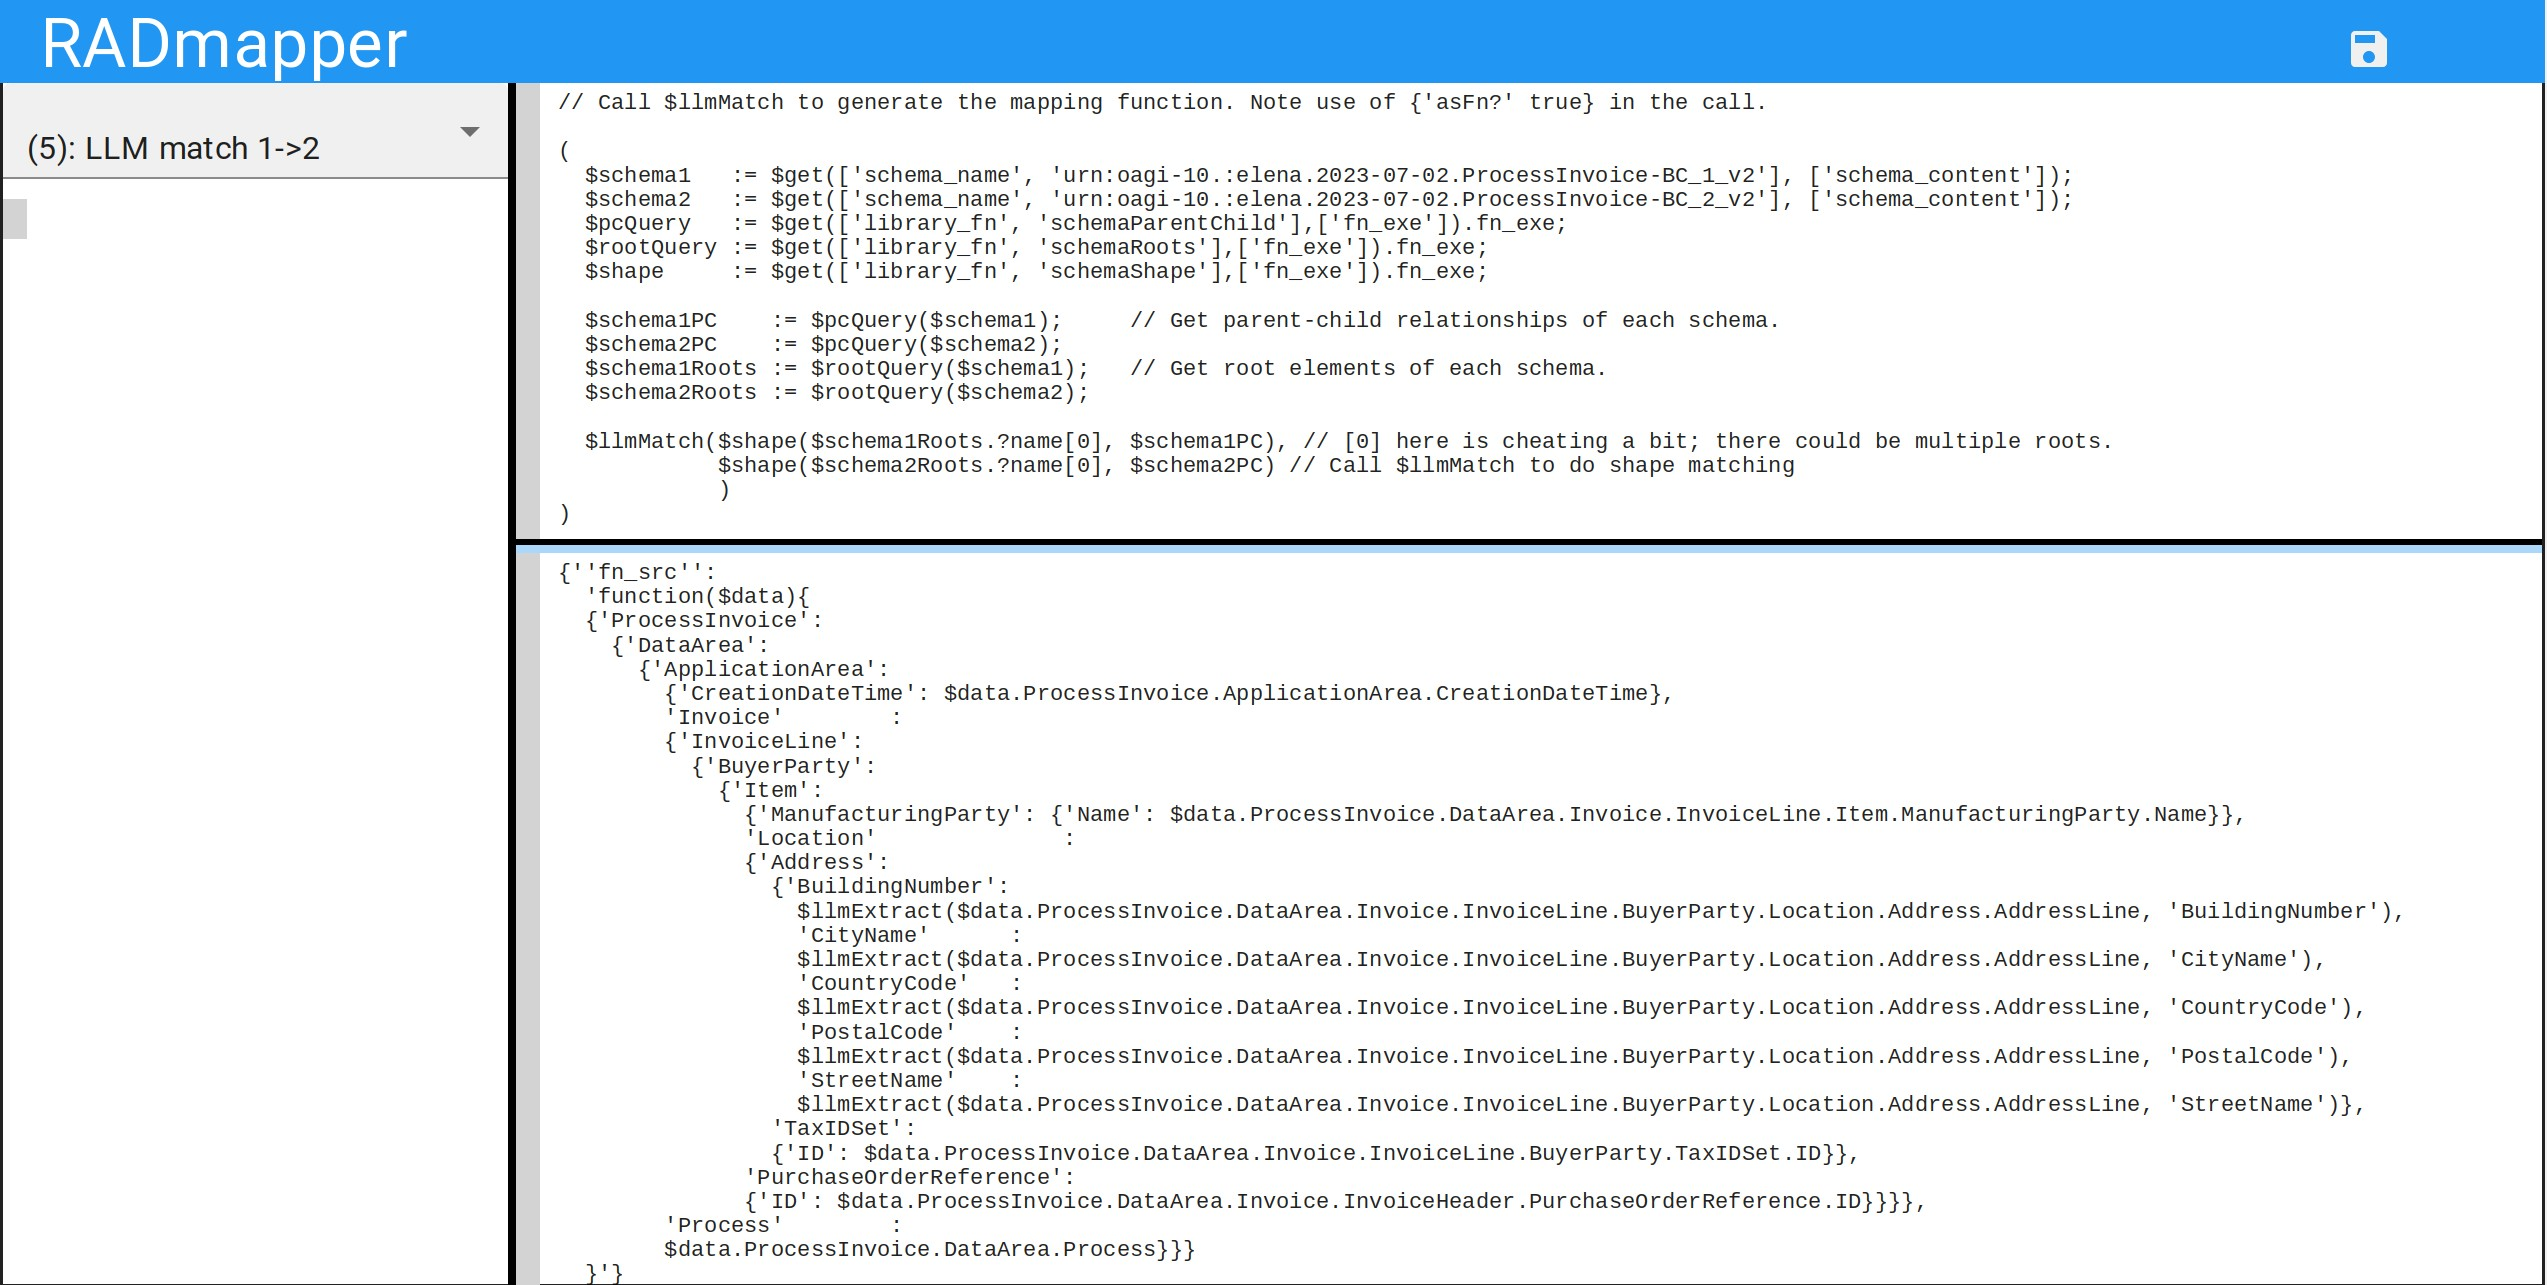
\includegraphics[scale=0.173]{RADmapperScreenshot.jpg}
\label{fig:RM-screenshot}
  \centering
\end{figure}


\section{Quick Start: Example Mapping Tasks}
\label{sec:quick-start}

This section uses examples to describe the basic features of the RADmapper language.
RADmapper provides the complete expression language and all the built-in functions of JSONata.
Like JSONata (and JavaScript) RADmapper is a functional language: functions can be passed to functions as values; the value returned from a function call can be a newly created function.
Examples of JSONata can be found in the JSONata specification. %\href{https://jsonata.org/}{JSONata specification}.
This section only goes into detail about the capabilities of RADmapper not found in JSONata.
The principal concepts to discuss are

\begin{itemize}
  \item{an end-to-end mapping task using Datalog, large language models, and the interoperable exchange form,}
  \item{the relational and graph forms of data,}
  \item{RADmapper's \stt{query} declaration, used to query relational data,}
  \item{RADmapper's \stt{express} declaration, used to reorganize (``map'') data from its original form to the form in which it is needed, and}
  \item{RADmapper's strategy for interoperable exchange of mapping specifications.}
\end{itemize}

\subsection{An End-to-end Example}

\subsubsection{Typical requirements}

Without going into detailed discussion about how things work, this section describes a mapping task end-to-end.
The example is typical of ``mapping'' problems: we have information encoded in one structure (the ``source'' form) and we'd like to express that information as another structure (the ``target'' form).
The example uses many of the capabilities of the RADmapper language and server capabilities of the exerciser\footnote{The exerciser can be viewed as a reference implementation for cases where you need executable to interact with a server.}, including
\begin{itemize}
  \item{fetching data,}
  \item{fetching stored functions,}
  \item{calling an LLM for matching and extraction,}
  \item{use of Datalog to query for data conforming to given patterns,}
  \item{human validation of AI-generated mapping functions.}
  \end{itemize}

The last bullet above, about validation, is in keeping with basic goals of RADmapper: we aim to produce results that express the essence of a mapping task in terms that are not so procedural looking that business-oriented analysts can't read them.\footnote{Or if we fall a little short of that goal, at least provide data for GUI tools that could illustrate what relationships are being asserted.}
Our guess is that, emerging AI capabililties notwithstanding, business-oriented validation is going to continue to be a requirement for the foreseeable future.
Thus, we aim for a result that is readable and easily serialized (as, say, JSON) so that it might be analyzed or translated into code for use with a commercial tool.

Let's suppose that you want to interact with a business partner using data the partner can easily provide.
You'd like your interface to accept the partner's form and map it to a form that your system can process directly.
Suppose the business partner's data are structured as suggested by the example In Figure~\ref{fig:data-for-end-to-end}, and that you'd like that information in a form shown beneath it in that figure.

% ToDo: It would have been good had I removed the extra "invoice" in these suckers.
% I would have to update fig:end-to-end-toAST too.
%\pagebreak
\begin{figure}[H]
  \caption{Example source and target data}
  \label{fig:data-for-end-to-end}
\begin{lstlisting}[language=JavaScript,numberstyle=\scriptsize,basicstyle=\ttfamily\scriptsize,numbers=left,stepnumber=1,breaklines=true]
// Example data you recieve from the partner:

{'Invoice':
  {'ApplicationArea':
    {'CreationDateTime': '2023-07-10'},
     'DataArea'       :
      {'Invoice':
        {'InvoiceHeader': {'PurchaseOrderReference': {'ID': 'PO-1234'}},
         'InvoiceLine'  : {'BuyerParty':
                            {'Location':
                              {'Address':
                                {'AddressLine':
                                  '123 Mockingbird Lane, Gaithersburg MD, 20878'}},
             'TaxIDSet': {'ID': 'tax-id-999'}},
           'Item'      : {'ManufacturingParty': {'Name': 'Acme Widget'}}}},
       'Process': 'Text description here, maybe.'}}}

// The form your system will accept:

{'Invoice':
  {'DataArea':
    {'ApplicationArea':
      {'CreationDateTime': '2023-07-10'},
      'Invoice'        :
        {'InvoiceLine':
          {'BuyerParty':
            {'Location':
              {'Address': {'BuildingNumber': '123',
                           'CityName': 'Gaithersburg',
                           'PostalCode': '20878',
                           'StreetName': 'Mockingbird Lane'}},
             'TaxIDSet': {'ID': 'tax-id-999'}},
            'Item'  :  {'ManufacturingParty': {'Name': 'Acme Widget'}},
            'PurchaseOrderReference': {'ID': 'PO-1234'}},
          'Process'    : 'Text description here, maybe.'}}}}
\end{lstlisting}
\end{figure} \vspace{-3em}

Two differences between the customer's form and yours are that, in your form:
\begin{enumerate}
\item{the customer's 'AddressLine' (Lines 12 and 13) is decomposed into its constituent details, BuildingNumber, CityName, (Lines 28--31) etc. in your target form and,}
\item{the customer's structure places the purchase order reference in a structure called InvoiceHeader (Line 8), whereas in your form a purchase order is associated with
each InvoiceLine, as shown by the nesting of Line 34 in the target structure.}
\end{enumerate}

\subsubsection{The function to do it}

Given examples of the data source and target in Figure~\ref{fig:data-for-end-to-end} it is not hard to see that the function in Figure~\ref{fig:mapping-src2tar} would get the job done;
it returns a structure that mirrors the target structure, and where it needs information from the source, it  describes paths into it.
Sometimes the paths are used directly, for example in Lines 5, 27, 29, 31, and 32.
Sometimes the data at the end of the path needs further processing.
On Lines 12, 16, 20 and 24, the paths are used in calls to  \stt{\$llmExtract} for such processing.
\stt{\$llmExtract} takes two arguments: a string (provided here by a path in the source data) and a term that describes a substring to be extracted from the string.\DIFaddbegin \footnote{\DIFadd{A few words about RADmapper syntax: (1) consistent with JSONata, RADmapper variables begin with a \$ and can be camelCase or use underscore, like \stt{\$my\_var}.
  Ordinary functions, including those that are defined by JSONata or RADmapper are bound to variables. 
  (2) The assignment operator is \stt{:=}.
  (3) The \stt{query} construct borrows syntactic features from Datalog-like languages.
  Specifically, \stt{query} variables begin with a question mark, \stt{?likeThis}, and role constants,
  which name attributes, begin with a colon and can contain underscore, for example, \stt{:element\_name}.
  (4) Note also that examples often depict strings delimited with single quote in JSON-like structures; legal JSON can also be generated.}}
\DIFaddend As you probably guessed from the name of the function, this function uses a large language model (LLM) to do the work.

\begin{figure}[H]
  \caption{A function that maps the source to target of Figure~\ref{fig:data-for-end-to-end}}
  \label{fig:mapping-src2tar}
\begin{lstlisting}[language=JavaScript,numberstyle=\scriptsize,basicstyle=\ttfamily\scriptsize,numbers=left,stepnumber=1,breaklines=true]
function($d){
 {'Invoice':
  {'DataArea':
    {'ApplicationArea':
      {'CreationDateTime': $d.Invoice.ApplicationArea.CreationDateTime},
      'Invoice'        :
      {'InvoiceLine':
        {'BuyerParty':
          {'Location':
            {'Address':
              {'BuildingNumber' :
                 $llmExtract(
                   $d.Invoice.DataArea.Invoice.InvoiceLine.BuyerParty.Location.Address.AddressLine,
                   'BuildingNumber'),
                'CityName'      :
                  $llmExtract(
                   $d.Invoice.DataArea.Invoice.InvoiceLine.BuyerParty.Location.Address.AddressLine,
                   'CityName'),
                'PostalCode'    :
                  $llmExtract(
                   $d.Invoice.DataArea.Invoice.InvoiceLine.BuyerParty.Location.Address.AddressLine,
                   'PostalCode'),
                'StreetName'    :
                  $llmExtract(
                   $d.Invoice.DataArea.Invoice.InvoiceLine.BuyerParty.Location.Address.AddressLine,
                   'StreetName')}},
            'TaxIDSet': {'ID': $d.Invoice.DataArea.Invoice.InvoiceLine.BuyerParty.TaxIDSet.ID}},
          'Item' : {'ManufacturingParty':
                      {'Name': $d.Invoice.DataArea.Invoice.InvoiceLine.Item.ManufacturingParty.Name}},
          'PurchaseOrderReference':
              {'ID': $d.Invoice.DataArea.Invoice.InvoiceHeader.PurchaseOrderReference.ID}},
        'Process' : $d.Invoice.DataArea.Process}}}}
  }
\end{lstlisting}
\end{figure} \vspace{-3em}

We could just leave things like this; it isn't hard (in this case) for a human to specify the paths shown above.
Further, were a human analyst to verify that the function above is what they need, then it is just a matter of turning the function into something easily exchanged (like JSON) to enable interoperable mapping.

Of course, it isn't hard to identify the mapping requirements expressed in Figure~\ref{fig:mapping-src2tar} using LLM tools either.
You could imagine, for example, LLM-based functions that recognize that CityName could be part of an AddressLine.
RADmapper contains such a function; it is called \stt{\$llmMatch}.
Below we show how it can be used to automatically generate functions like the one in Figure~\ref{fig:mapping-src2tar}.

\subsubsection{A methodology around ``the function to do it''}

A mapping methodology deployable at enterprise scale might use a three-step process for generating and using
mapping functions like the one in Figure~\ref{fig:mapping-src2tar}:
\begin{description}
  \item[Step A] Compute the abstract ``shape'' of the source and target structures, such as those in Figure~\ref{fig:data-for-end-to-end}.
  \item[Step B] Provide these shapes to an LLM function, \stt{\$llmMatch}, to reconcile differences in the source and target structures, generating functions for mapping between them.
\item[Step C] Verify, document, and store the generated function for use whenever this type of mapping is needed.
\end{description}

We will start by discussing the ``store the generated function'' part of Step C because it involves basic capabilities used in Step A.
RADmapper has store and retrieve functions \stt{\$put}, and \stt{\$get} that work the same on data and functions.
We can demonstrate use of the stored function with the exerciser web app.
In your tooling, you might access the data and function much differently.
In the exerciser, it looks like Figure~\ref{fig:run-a-map-fn} below.\footnote{This example is currently executable from the exerciser https://hub.docker.com/r/podenno/rm-exerciser as the default example, if you'd like to try it yourself.
  Note that the exerciser has an OpenAPI (swagger) interface.
  In the exerciser docker image, it is documented at http://localhost:3000; the app itself is http://localhost:3000/app.}

\begin{figure}[H]
  \caption{Suppose that using Step B of the three-step process we created a mapping function, \stt{invoice-match-1->2-fn}, and using Step C we validated and stored it.
    In this code, we are \stt{\$get}-ing and using it.}
  \label{fig:run-a-map-fn}
\begin{lstlisting}[language=JavaScript,numberstyle=\scriptsize,basicstyle=\ttfamily\scriptsize,numbers=left,stepnumber=1,breaklines=true]
(
  $data := $get(['library_fn', 'bie-1-data'], ['fn_exe']).fn_exe;
  $mappingFn := $get(['library_fn', 'invoice-match-1->2-fn'], ['fn_exe']).fn_exe;
  $mappingFn($data)
)
\end{lstlisting}
\end{figure} \vspace{-3em}

Line 2 of this example calls \stt{\$get} to get the example data.
\stt{\$get} works something like GraphQL, in this case just specifying one property of the argument object, \stt{['library\_fn', 'bie-1-data']}, to retrieve.
Running from the exerciser, \stt{\$get} is an async call to the server serving the app.
Line 3 similarly gets the mapping function. Note that both lines (and indeed the whole example and most RADmapper syntax) conforms to JSONata syntax.
\stt{\$get} returns an object with the attributes listed in its second argument.
Both Line 2 and Line 3, use JSONata syntax, \stt{.fn\_exe}, to get the one property retrieved from the object, its executable.\footnote{You are probably wondering what ``getting the executable'' means with respect to  data such as Line 2 in Figure~\ref{fig:run-a-map-fn}.
  These \stt{'library\_fn'} objects have three attributes, \stt{fn\_exe}, \stt{fn\_src}, and \stt{fn\_doc},
  each of which are strings.
  In the case of data, \stt{fn\_exe} returns the structure represented by that string, just as you might do with a string representing JSON.}
Line 4 applies the \stt{\$mappingFn} to the \stt{\$data} resulting in an object like shown in Lines \DIFdelbegin \DIFdel{of }\DIFdelend 20--35 of Figure~\ref{fig:data-for-end-to-end}.

Now let's talk about about Step A, creating the shape structures.
The shape structures are simply nested objects typical of example data where the non-object content is replaced by the string \stt{'<data>'}.
For example,

\begin{lstlisting}[language=JavaScript,numbers=none,basicstyle=\ttfamily\scriptsize]
      {'Invoice':
        {'InvoiceHeader': {'PurchaseOrderReference': {'ID': '<data>'}},
         'InvoiceLine'  : {'BuyerParty':
                             {'Location':
                               {'Address': {'AddressLine': '<data>'}},
                              'TaxIDSet': {'ID': '<data>'}},
                           'Item' :
                             {'ManufacturingParty': {'Name': '<data>'}
                              'ItemDescription'   : '<data>'}}}.
\end{lstlisting} \vspace{-2em}
Of course, you could create things like this by typing them in, but, so as to illustrate the use of a RADmapper function-like construct \DIFaddbegin \DIFadd{like }\DIFaddend \stt{query}, we will assume there are schema defining these structures; we'll use a Datalog-like \stt{query} to create the structures. The code to do this is a bit involved; it would be saved as a function and applied, but for the sake of exposition we'll discuss the whole thing, shown below.
Just keep in mind that this is not part of the much simpler process of doing the three steps.
Here we are looking behind the curtain.

\begin{figure}[H]
  \caption{Details of the process of creating shape data from source and target schema for invoices.
    In practice, you might make a function from this to hide such detail.}
  \label{fig:def-of-shape-fn}
\begin{lstlisting}[language=JavaScript,numberstyle=\scriptsize,basicstyle=\ttfamily\scriptsize,numbers=left,stepnumber=1,breaklines=true]
( // This code shows all the detail of creating shapes for $llmMatch.

  $schema1 := $get(['schema_name', 'urn:oagi-10.:elena.2023-07-02.ProcessInvoice-BC_1_v2'], ['schema_content']);
  $schema2 := $get(['schema_name', 'urn:oagi-10.:elena.2023-07-02.ProcessInvoice-BC_2_v2'], ['schema_content']);

  $pcQuery := query{[?x     :element_name        ?parent] // pc = 'parent/child'
                    [?x     :element_complexType ?cplx1]
                    [?cplx1 :model_sequence      ?def]
                    [?def   :model_elementDef    ?cplx2]
                    [?cplx2 :element_name        ?child]};

  $rootQuery := query{[?c :schema_content   ?e]
                      [?e :model_elementDef ?d]
                      [?d :element_name     ?name]};

  // This function just gets the children for a parent.
  $children := function($spc, $p) { $spc[?parent = $p].?child };

  // This function calls itself recursively to build the schema shape, starting from the root.
  $shape :=
    function($p, $spc)
      { $reduce($children($spc, $p),
                function($tree, $c) // Update the tree.
                  { $update($tree,
                            $p,
                            function($x) { $assoc($x, $c, $lookup($shape($c, $spc), $c) or '<data>')}) },
                {})};

  $schema1PC    := $pcQuery($schema1);     // Call the two queries with the two schema.
  $schema2PC    := $pcQuery($schema2);     // The first two return a binding set for {?parent x ?child y}
  $schema1Roots := $rootQuery($schema1);   // The last two return a binding set for {?name} (of a root).
  $schema2Roots := $rootQuery($schema2);

  {'shape1' : $shape($schema1Roots.?name[0], $schema1PC),
   'shape2' : $shape($schema2Roots.?name[0], $schema2PC)}
)
\end{lstlisting}
\end{figure} \vspace{-3em}

We'll walk through this code line by line:
\begin{description}
\item[Lines 3 and 4, \$get:]
  These lines get the schema objects, which are big and contain lots of information superfluous to our goals.
  So we won't discuss them further here.
\DIFdelbegin %DIFDELCMD < \item[Lines 6-14, query:]
\item[\DIFdel{Lines 6-14, query:}]%DIFAUXCMD
%DIFDELCMD <   %%%
\DIFdel{These are definitions of query constructs }\DIFdelend \DIFaddbegin \item[\DIFadd{Lines 6--10, parent/child query:}]
  \DIFadd{The query construct, }\DIFaddend described further in Section~\ref{sec:query}\DIFdelbegin \DIFdel{;
  they define functions }\DIFdelend \DIFaddbegin \DIFadd{, defines a function }\DIFaddend that provide Datalog-like capabilities.
  \DIFdelbegin \DIFdel{Corresponding to the \bdef{role definitions} like \stt{:element\_name} on Line 6,
  there is somewhere in the structures assigned to \stt{\$schema1} and \stt{\$schema1}
  object attributes \stt{'element\_name'} which, when this query is applied to that schema will produce a structure that binds \stt{?parent} to the element name (and so on for other object attributes).
  \stt{query} will be discussed in detail in later examples.
  Lines 6--10 define the query functionfor finding parent}\DIFdelend \DIFaddbegin \DIFadd{This code binds \stt{\$pcQuery} to a function that collects a certain kind of parent}\DIFaddend /child relationships in the schema data,
  \DIFaddbegin \DIFadd{specifically, those that relate an entity bound to \stt{?parent} to an entity bound to \stt{?child} through
  the navigation of roles shown(from the entity bound to \stt{?x} through its \stt{element\_complexType} attribute, to a \stt{model\_sequence}, to \stt{model\_elementDef}
  Note that the function is then used on Lines 29 }\DIFaddend and \DIFaddbegin \DIFadd{30.
%DIF >   Corresponding to \bdef{role definitions} like \stt{:element\_name} on Line 6, there is somewhere in the structures assigned to \stt{\$schema1} and \stt{\$schema1}
%DIF >   object attributes \stt{'element\_name'} which, when this query is applied to that schema will produce a structure that binds \stt{?parent} to the element name (and so on for other object attributes).
%DIF >   \stt{query} will be discussed in detail in later examples.
}\item [\DIFaddend Lines 12--14\DIFdelbegin \DIFdel{define the query function for finding the root elements in the schema}\DIFdelend \DIFaddbegin \DIFadd{, root query:}]  \DIFadd{Similar to Lines 6--10 this code define a query function.
  Owing to the structure of the }\DIFaddend data\DIFaddbegin \DIFadd{, there is only one object, \stt{?c}, with a \stt{schema\_content} attribute.
  That object binds the values of \stt{schema\_content} to \stt{?e} and Lines 13 and 14 follow a navigation
  resulting in a binding in the element names of root elements of the schema}\DIFaddend .
\item[Line 17, parent/child function:] Defines a small function to return the children of a parent.
\item[Lines 20--27, shape function:] Defines a function to create the shape structures.
  This uses two RADmapper functions not found in JSONata.
  \stt{\$assoc} takes an object, an attribute and a value and installs the value at that attribute in the object.
  \stt{\$update} is similar but calls the 3rd argument function on the value in the attribute to update it.\footnote{
    Though the names  \stt{\$assoc} and  \stt{\$update} might sound like they modify data, they are pure functions, creating new objects.} This function is the behind-the-curtain kind of thing we were warning you about.
\item[Lines 29--32, function calls:] These call the parent/child and root functions to get arguments for the call to the \stt{\$shape} function.
\item[Lines 34--35, function calls:] Presentation of the results of calling the \stt{\$shape} function on the two schema are (in either order)
  source and target shapes for calls to \stt{\$llmMatch}.
\end{description}

As will be discussed in Section~\ref{sec:query}, \stt{query} offers means to treat object structures as though they were were databases;
it thereby offers an alternative to Xpath-like JSONata for manipulating data.
The \textit{binding set} that is the returned value of \stt{query} calls are especially useful when calling \stt{\$reduce} on a \stt{express} function/structure, as will be demonstrated in later examples.

\begin{figure}[H]
  \caption{Code to perform Step A, calling the shape function, and Step B, using the shapes to create a mapping function.
  Note that Lines 6--8 suggests that functions such as the one in Figure~\ref{fig:def-of-shape-fn} were stored as library functions.}
  \label{fig:call-to-shape}
\begin{lstlisting}[language=JavaScript,numberstyle=\scriptsize,basicstyle=\ttfamily\scriptsize,numbers=left,stepnumber=1,breaklines=true]
// Call $llmMatch to generate the mapping function. Note use of {'asFn?' true} in the call.

(
  $schema1   := $get(['schema_name', 'urn:oagi-10.:elena.2023-07-02.ProcessInvoice-BC_1_v2'], ['schema_content']);
  $schema2   := $get(['schema_name', 'urn:oagi-10.:elena.2023-07-02.ProcessInvoice-BC_2_v2'], ['schema_content']);
  $pcQuery   := $get(['library_fn', 'schemaParentChild'],['fn_exe']).fn_exe;
  $rootQuery := $get(['library_fn', 'schemaRoots'],['fn_exe']).fn_exe;
  $shape     := $get(['library_fn', 'schemaShape'],['fn_exe']).fn_exe;

  $schema1PC    := $pcQuery($schema1);     // Get parent-child relationships of each schema.
  $schema2PC    := $pcQuery($schema2);
  $schema1Roots := $rootQuery($schema1);   // Get root elements of each schema.
  $schema2Roots := $rootQuery($schema2);

  $llmMatch($shape($schema1Roots.?name[0], $schema1PC), // [0] is cheating a bit; there could be multiple roots.
            $shape($schema2Roots.?name[0], $schema2PC), // Call $llmMatch to do shape matching
            {'asFn?' : true})
)
\end{lstlisting}
\end{figure} \vspace{-3em}

Note that in Line 17 of Figure~\ref{fig:call-to-shape} the call to \stt{\$llmMatch} specifies the options \stt{\{'asFn?' : true\}}. This is used to specify that \stt{\$llmMatch} is to return a structure containing function source.
That source is what is depicted in Figure~\ref{fig:mapping-src2tar}.
If in testing (Step C verification) the function proves fit for purpose, it can be documented and stored.
It could also be communicated to others in interoperable form using the function \stt{\$toAST}, which is discussed in Section~\ref{sec:toAST}.

\section{Data Organized as Triples}
 \label{sec:query}

\subsection{Constructing binding sets with \stt{query}}

\stt{query} is the principal construct of RADmapper providing Datalog-like functionality to the language.\footnote{
  If you know SPARQL, Datalog will look familiar.}
%You first saw it in Figure~\ref{fig:def-of-shape-fn}.
\stt{query} declarations are used like JSONata or JavaScript function declaration in the sense that the value of the declaration (a function) can be assigned to variables and used directly.
For example,
\begin{lstlisting}[language=JavaScript,numbers=none,basicstyle=\ttfamily\scriptsize]
$addOne := function(x){x + 1}
\end{lstlisting} \vspace{-2em}
defines a function and assigns it to the variable \stt{\$addOne}.
\stt{\$addOne(3)} is a call to the function with the argument 3.
Similarly,
\begin{lstlisting}[language=JavaScript,numbers=none,basicstyle=\ttfamily\scriptsize]
$myQuery := query(){[$DB1 ?person :age 42]}
\end{lstlisting} \vspace{-2em}
defines a query that can be used like a function.
\stt{\$myQuery(\$myDB)} is a call to the function with whatever ``database'' is assigned to \stt{\$myDB}.
However, unlike ordinary functions, the body of a \stt{query} consists of one or more \bdef{Datalog patterns}, such as the \stt{[\$DB1 ?person :age 42]} above.
We'll start by talking about the database argument to the query, for example, the value assigned to \stt{\$MyDB} in the expression \stt{\$myQuery(\$MyDB)} then get back to talking about the patterns.

Graph-based data (and 5th-form normalized relational data) can be described by triples $[x,rel,y]$ where $x$ is an entity reference, $y$ is data (string, number, entity reference, etc.) and $rel$ is a relationship (predicate or edge name) holding between $x$ and $y$.
For example, in syntax similar to JSON we could describe the fact that Bob's age is 42 with an object \stt{\{'name' : 'Bob', 'age' : 42\}}.
As triples, we represent Bob being 42 years old with two triples, for example, \stt{[152 'name' 'Bob']} and \stt{[152 'age' 42]}.
As a graph, this would look like the following:

\begin{figure}[H]
  \caption{Information about Bob in graph form\DIFaddbeginFL \DIFaddFL{.}\DIFaddendFL }
  \label{fig:bob-as-a-graph}
     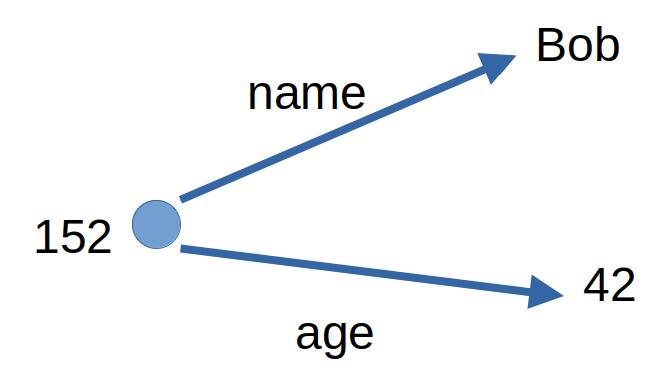
\includegraphics[scale=0.15]{bob-age-42.jpg}
  \centering
\end{figure}

You might wonder where the 152 in the triples came from, or for that matter, why the fact that Bob being age 42 couldn't
simply be represented by the single triple \stt{['Bob' 'age' 42]}.
The answer is that you could represent this fact with that one triple, but in doing so you are using \stt{'Bob'} as a key
which might not be that good if your database has more than one Bob in it.
So instead, to prepare for the more general case, Datalog-like graph databases use integers to refer to entities.
152 here is like a primary key in relational DB, or an IRI for a particular entity defined in RDF.
A complete RADmapper program for querying the Bob database for people age 42 is as follows:

\begin{figure}[H]
  \caption{A complete query.}
  \label{code:bob-age}
\begin{lstlisting}[language=JavaScript,numberstyle=\scriptsize,basicstyle=\ttfamily\scriptsize,numbers=left,stepnumber=1,breaklines=true]
 ( $myDB := [{'name' : 'Bob', 'age' : 42}];
   $ageQuery := query(){[?e :age 42]};
   $result := $ageQuery($myDB); )
\end{lstlisting}
\end{figure} \vspace{-3em}

% ToDo: I think I made a mistake by calling the thing returned by query a binding set. It is a collection of binding sets.
%       Or maybe binding element was the problem. But element and set are wrong. I should call the each one a binding object
%       where "object" means "dictionary" (python) or the JS notion of object. "A collection of binding objects"
%       In the code I can call it whatever. Keep it binding set, I think.
%       Even this isn't very good! +Maybe check what Abiteboul called it.+ ... They don't.
%       See https://en.wikipedia.org/wiki/Datalog.
% 2024-09-27: I finally settled on "binding object" and "binding set".


The above needs some explanation.
On Line 1 we put a JSON-like object in \DIFdelbegin \DIFdel{an }\DIFdelend \DIFaddbegin \DIFadd{a }\DIFaddend JavaScript-like array by wrapping it in square brackets; this is the literal form of a very small database.
On Line 2 we defined the query function; here note the use of a \bdef{query variable} \stt{?e}.
Also note that whereas we used the string \stt{'age'} for the relation, we used \stt{:age} --- syntax we call an \bdef{attribute} --- to represent that same relation in the pattern.
On Line 3 we apply the query function \stt{\$ageQuery} to the database \stt{\$myDB} defined on Line 1.
Of course, \stt{\$myDB} isn't much of a database; it contains only the data shown in Figure~\ref{fig:bob-as-a-graph}.
Alternatively, you could have defined data through other means, such as reference to a file or a GraphQL query.
The result of this query, assigned to \stt{\$result} is a collection of \bdef{binding objects}, where each
object associates values to pattern variables (object keys) from the \stt{query} consistent with the database.
In this example, with the data in Figure~\ref{fig:bob-as-a-graph}, the result consists of just one binding object and that object binds one variable;
thus, the \bdef{binding  set} is the one-element set \stt{[\{?e : 152\}]}.\footnote{Binding sets are mathematical sets. Binding objects binding the same variables to the same objects are values \DIFdelbegin \DIFdel{; they }\DIFdelend describe the same navigation of the database.}
This indicates that the entity indexed at 152 has an attribute \stt{:age} with value 42.
If there were more entities in the database possessing an \stt{:age} attribute, the query would have returned a set consisting of one such \stt{\{?e : <whatever>\}} binding object for each of them.

Amazing as that query might seem, running against a database with one entity in it and all, it didn't tell us the names of persons age 42.
All we got was a binding object for every entity that has an age attribute equal to 42.
Entity IDs are internal to the database and not of much value to RADmapper users.\footnote{In fact, I sort of told a fib for ease of exposition; by default the binding of variables in the entity position, entity ID integers, are not provided in binding objects.
  Using default settings, what this example returns is \stt{[\{\}]} meaning ``one match was found.''
The binding sets depicted in most examples won't include bindings for entity IDs.}
In order to make any use of this information, we need to join the \stt{[?e :age 42]} pattern with a pattern that grabs the name attribute in the data, \stt{[?e :name ?name]}.
This is shown in Figure~\ref{code:bob-age-more} below.

\begin{figure}[H]
    \caption{A more useful query, getting the names of 42-year old persons.}
    \label{code:bob-age-more}
\begin{lstlisting}[language=JavaScript,numberstyle=\scriptsize,basicstyle=\ttfamily\scriptsize,numbers=left,stepnumber=1,breaklines=true]
 ( $myDB := [{'name' : 'Bob', 'age' : 42}];
   $ageQuery := query(){[?e :age 42]
                        [?e :name ?name]}
   $result := $ageQuery($myDB); )
\end{lstlisting}
\end{figure} \vspace{-3em}

The pattern on Line 3, by virtue of its reuse of \stt{?e}, imposes an additional constraint on the graph match: the entity bound to \stt{?e} must have a \stt{:name} attribute.
The value of the name attribute is bound to \stt{?name}.
Thus each binding object in the binding set will bind two variable, \stt{?e} and \stt{?name}.
The binding set for the database in the graph depicted in Figure~\ref{fig:bob-as-a-graph} is \stt{[\{?e : 152, ?name 'Bob'\}]}.\footnote{If you read the previous footnote you know it actually returns just \stt{[\{?name 'Bob'\}].}}

In this example, we used one variable to match on the entity and another to capture a value, however each position (entity, attribute, and value) can take a variable.
Further, you can use variables in more than one of those positions.
For example, \stt{query()\{[?entity ?attr ?val]\}} is a query that matches on every entity, attribute, and value of the database; it represents every edge of the database's graph.
\stt{query\{[\_ ?attr \_]\}} would return the names of all the attributes in the database (without duplicates). % ToDo: Fix this in the code!
This provides a kind of introspection that is typically more difficult to obtain in other database technology.
When matching the value position you are doing a relational join, for example, we might match the social security number (SSN) in
some data against a same-valued (but possibly differently named) value in other data.
For example,

% ToDo: Get rid of numbering on this example.
\begin{lstlisting}[language=JavaScript,numbers=none,basicstyle=\ttfamily\scriptsize]
   $relJoinQuery := query(){[$DB1 ?e1 :ssn ?id]
                            [$DB2 ?e2 :id  ?id]}
\end{lstlisting} \vspace{-2em}

You may have noticed that the query above, and one used earlier have four elements in their pattern whereas most of the examples have only three (entity, attribute, and value).
If four elements are provided, the first is the database to which the pattern is applied.
If there is only one database being queried, as we've been doing earlier, you do not need to use four-place patterns.
Let's look at a complete \stt{query} example that uses two databases.

\begin{figure}[H]
    \caption{A query that joins information from two databases}
    \label{code:two-database-query}
\begin{lstlisting}[language=JavaScript,numberstyle=\scriptsize,basicstyle=\ttfamily\scriptsize,numbers=left,stepnumber=1,breaklines=true]
( $DBa := [{'email' : 'bob@example.com', 'aAttr' : 'Bob-A-data',   'name' : 'Bob'},
           {'email' : 'alice@alice.org', 'aAttr' : 'Alice-A-data', 'name' : 'Alice'}];
  $DBb := [{'id'    : 'bob@example.com', 'bAttr' : 'Bob-B-data'},
           {'id'    : 'alice@alice.org', 'bAttr' : 'Alice-B-data'}];

  $qFn :=  query(){[$DBa ?e1 :email ?id]
                   [$DBb ?e2 :id    ?id]
                   [$DBa ?e1 :name  ?name]
                   [$DBa ?e1 :aAttr ?aData]
                   [$DBb ?e2 :bAttr ?bData]};

  $bSet := $qFn($DBa, $DBb);  )
\end{lstlisting}
  \end{figure} \vspace{-2em}

  In Figure~\ref{code:two-database-query} Lines 1--4 we define two small databases and assign them to variables \stt{\$DBa} and \stt{\$DBb} respectively. On Lines 6--10 we define the query.
Since both databases use email addresses for customer identification, we can use the \stt{:email} and \stt{:id} attributes to join together information about a customer from the two databases.
That is the purpose of the patterns on Lines 6 and 7; the two patterns use different variables for the entities, \stt{?e1} and \stt{?e2},
because the information is coming from different databases and we do not control entity IDs, but both use \stt{?id} to force
matches on email address.
The remainder of the patterns in the query, Lines 8--10, pick up various information from the two databases.
Line 12 calls the query function bound to \stt{\$bSet} to get the binding set against the two databases.
Unlike our previous calls to the query function, this one takes two databases as arguments.
The order of the arguments in the call must be the same as the order in which the databases appear in the query statement;
\stt{\$DBa} appears first on Line 6, \stt{\$DBb} appears first on Line 7, so \stt{\$DBa} is the first argument to the call.

The binding set that is produced, the value of \stt{\$bSet}, consists of two binding objects:

\begin{lstlisting}[language=JavaScript,numbers=none,basicstyle=\ttfamily\scriptsize]
[{?id : "bob@example.com", ?name : "Bob",   ?aData : "Bob-A-data",   ?bData : "Bob-B-data"  },
 {?id : "alice@alice.org", ?name : "Alice", ?aData : "Alice-A-data", ?bData : "Alice-B-data"}]
\end{lstlisting} \vspace{-2em}

One small but very significant point before moving on to discuss \stt{express}:
writing queries like \stt{query()\{[?e :age 42] [?e :name ?name]\}} could become rather tedious in the case that you might want to get data about some other age value.
For this reason, the \stt{query} declaration can serve to produce a higher-order function, a function that returns (query) functions as values. Figure~\ref{code:higher-order-query} demonstrates the idea.

% ToDo: Should I allow jvars to be the keys of binding sets, and thereby eliminate the need for such things as [?e :age ?age] below?

\begin{figure}[H]
    \caption{Get the names of people ages 42 and 33.}
    \label{code:higher-order-query}
\begin{lstlisting}[language=JavaScript,numberstyle=\scriptsize,basicstyle=\ttfamily\scriptsize,numbers=left,stepnumber=1,breaklines=true]
 ( $myDB := [{'name' : 'Bob',   'age' : 42},
              'name' : 'Alice', 'age' : 33}]

   $ageQueryT := query($age){[?e :age  $age]
                             [?e :age  ?age]
                             [?e :name ?name]}

   $ageQ42    := $ageQueryT(42);
   $ageQ33    := $ageQueryT(33);

   $append($ageQ42($myDB) , $ageQ33($myDB))  )
\end{lstlisting}
\end{figure} \vspace{-3em}

The key difference is that on Line 4, the \stt{query} construct, defines a parameter, \stt{\$age}, using ordinary JSONata-like syntax.
You can define as many parameters as you'd like and they can be used to substitute into any of the pattern positions, entity, attribute, or value.
By convention, if we are to assign a higher-order \stt{query} function to a variable, we end the variable name with a \stt{T} such as shown on Line 4, \stt{\$ageQueryT}.
The T suggests that the variable denotes a \bdef{query template}.
Lines 8 and 9 define query functions for querying ages 42 and 33, respectively.
Line 11 uses the JSONata-like builtin \stt{\$append} to combine the two binding sets.
Note that the pattern \stt{[?e :age ?age]} on Line 5 is used get ?age into the binding sets.
The result of running this example is the binding set

\begin{lstlisting}[language=JavaScript,numbers=none,basicstyle=\ttfamily\scriptsize]
  [{?name : 'Bob',   ?age : 42},
   {?name : 'Alice', ?age : 33}].
\end{lstlisting} \vspace{-2em}

\subsection{Constructing  Target Data with \stt{express}}

Binding sets produced by \stt{query} provide ordinary JSONata-like objects\footnote{Two differences: (1) the keys of binding objects are query variables, and (2) binding objects are always flat objects; the values at the keys are not objects themselves though they may be entity IDs (integers) referencing objects. These differences notwithstanding, you can use binding objects as though they are ordinary JSONata-like objects.} that could be used with JSONata built-in functions and operators to produce target structures.
However, the \stt{express} construct provides capabilities beyond those of the JSONata expression language.
This section describes some of those features.

Let's continue with our two-database example.
Lines 1--12 of Figure~\ref{code:two-database-query-express} below are as they were in Figure~\ref{code:two-database-query}.
The binding set assigned to \stt{\$bSet} is
\begin{lstlisting}[language=JavaScript,numbers=none,basicstyle=\ttfamily\scriptsize]
[{?id : "bob@example.com", ?name : "Bob",   ?aData : "Bob-A-data",   ?bData : "Bob-B-data"  },
 {?id : "alice@alice.org", ?name : "Alice", ?aData : "Alice-A-data", ?bData : "Alice-B-data"}].
\end{lstlisting} \vspace{-2em}

Assuming that we'd just like to present the target data as nested objects indexed by the customer's email address, for example:

\DIFmodbegin
\begin{lstlisting}[language=JavaScript,numbers=none,basicstyle=\ttfamily\scriptsize,alsolanguage=DIFcode]
%DIF < {"alice@alice.org" {"name"  : "Alice",
%DIF > {"alice@alice.org" : {"name"  : "Alice",
                      "aData" : "Alice-A-data",
                      "bData" : "Alice-B-data" },

%DIF <  "bob@example.com" {"name"  : "Bob",
%DIF >  "bob@example.com" : {"name"  : "Bob",
                      "aData" : "Bob-A-data",
                      "bData" : "Bob-B-data"   }}
\end{lstlisting}
\DIFmodend \vspace{-2em}

\hspace{-2em} we could use the \stt{express} declaration that begins on Line 14 of Figure~\ref{code:two-database-query-express} to do this.

\begin{figure}[H]
    \caption{Using express with a query that looks into two databases}
    \label{code:two-database-query-express}
\begin{lstlisting}[language=JavaScript,numberstyle=\scriptsize,basicstyle=\ttfamily\scriptsize,numbers=left,stepnumber=1,breaklines=true]
( $DBa := [{'email' : 'bob@example.com', 'aAttr' : 'Bob-A-data',   'name' : 'Bob'},
           {'email' : 'alice@alice.org', 'aAttr' : 'Alice-A-data', 'name' : 'Alice'}];
  $DBb := [{'id'    : 'bob@example.com', 'bAttr' : 'Bob-B-data'},
           {'id'    : 'alice@alice.org', 'bAttr' : 'Alice-B-data'}];

  $qFn := query(){[$DBa ?e1 :email ?id]
                  [$DBb ?e2 :id    ?id]
                  [$DBa ?e1 :name  ?name]
                  [$DBa ?e1 :aAttr ?aData]
                  [$DBb ?e2 :bAttr ?bData]};

  $bSet := $qFn($DBa, $DBb);

  $eFn  := express(){{?id : {'name'  : ?name,
                             'aData' : ?aData,
                             'bData' : ?bData}}};

  $reduce($bSet, $eFn) )
\end{lstlisting}
\end{figure} \vspace{-3em}

\stt{express} is a function-defining construct that, like \stt{query}, is capable of returning express functions when supplied with parameters.
In that sense, it is capable of being a higher-order function.
But here on Line 14 we are not using parameter; the declaration is simply \stt{express()\{...\}}; no parameters imply it isn't a template and can be used directly.
The body of the \stt{express} declaration, the text inside the outer curly brackets, defines the pattern of JSONata-like object structure.
The target data is produced by iterating over the express function bound to \stt{\$eFn} using the elements of the binding set.
Two of the most common ways to iterate over a function in functional languages such as JSONata and RADmapper are map and reduce.
Map and reduce differ in how they process the collection of arguments:
map applies a given function to each element independently;
reduce ``summarizes'' results by allowing each element to replace an on-going structure with an updated one.\footnote{Examples to help you recall how these work:
  \\ \stt{\$map([1,2,3,4], function(\$x)\{\$x * 2\})} returns [2,4,6,8]; it multiplies each argument by 2.
  \\ \stt{\$reduce([1,2,3,4], function(\$x, \$y)\{\$x + \$y\})} returns 10; it applies \stt{+} to 1 and 2, then to 3 and that sum,
  then to 4 and that sum.}
Whether you \stt{\$map} or \stt{\$reduce} the \stt{express} function over the binding set can have great influence on the outcome, as will be demonstrated in subsequent examples.
As written above, the call to \stt{\$reduce} on Line 18 creates a nested structure for the first binding object and then inserts a second structure into it at the second \stt{?id} key, as shown above.
Were Line 18 replaced with \stt{\$map(\$bSet, \$eFn)}, the result would be two independent nested maps, one for each binding object in the call to \stt{\$map}:

\begin{lstlisting}[language=JavaScript,basicstyle=\ttfamily\scriptsize,numbers=none]
[{"bob@example.com" : {"name" : "Bob",   "aData" : "Bob-A-data",  "bData" : "Bob-B-data"  }},
 {"alice@alice.org" : {"name" : "Alice", "aData" : "Alice-A-data","bData" : "Alice-B-data"}}].
\end{lstlisting} \vspace{-2em}

\subsection{Example use of  \stt{query}  and  \stt{express} }

This example illustrates (1) simple restructuring of a data structure, (2) use of predicates as query patterns, (3) extensive joining
to navigate deeply nested structures, and (4) use of query variable in the attribute position of patterns.
The example is based on a discussion on the JSONata Slack channel.
The goal of the example is to swap the nesting of \stt{owners} and \stt{systems} as shown in Figure~\ref{data:restruct}.

\begin{figure}[H]
  \caption{The goal is to swap the nesting of ``owners'' and ``systems'' in the data on Lines 1--9  so that it looks Lines 13--21.}
 \label{data:restruct}
\begin{lstlisting}[language=JavaScript,basicstyle=\ttfamily\scriptsize,numberstyle=\scriptsize]
{ "systems":
   { "system1": { "owners": { "owner1": { "device1": { "id": 100, "status": "Ok" },
                                          "device2": { "id": 200, "status": "Ok" }},
                              "owner2": { "device3": { "id": 300, "status": "Ok" },
                                          "device4": { "id": 400, "status": "Ok" }}}},
     "system2": { "owners": { "owner1": { "device5": { "id": 500, "status": "Ok" },
                                          "device6": { "id": 600, "status": "Ok" }},
                              "owner2": { "device7": { "id": 700, "status": "Ok" },
                                          "device8": { "id": 800, "status": "Ok" }}}}}}

 /* ...so that it looks like: */

{"owners":
   {"owner1": {"systems": {"system1": {"device1": {"id": 100, "status": "Ok"},
                                       "device2": {"id": 200, "status": "Ok"}},
                           "system2": {"device5": {"id": 500, "status": "Ok"},
                                       "device6": {"id": 600, "status": "Ok"}}},
    "owner2": {"systems": {"system1": {"device3": {"id": 300, "status": "Ok"},
                                       "device4": {"id": 400, "status": "Ok"}},
                           "system2": {"device7": {"id": 700, "status": "Ok"},
                                       "device8": {"id": 800, "status": "Ok"}}}}}))))
\end{lstlisting}
\end{figure} \vspace{-3em}

%Though these structures, rendered as JSON, may look odd (for example, there are no arrays used despite apparent value in having %them\footnote{For example, several devices are associated with an owner, but instead of arrays, the developer used meaningful names as keys, %"device1","device2" etc. Perhaps these structures seems unusual because they don't allow you to write code to get data using fixed names.
%  Except for ``owners'', and ``systems'', the rest are enumerating things; it requires a sort of ``positional semantics''. }) this is not %relevant to the discussion.
Typical of a restructuring task, the goal data on Lines 13--21 does not contradict any of the facts evident in the original data on Lines 1--9.
For example, there is an owner called \stt{owner1}, and \stt{owner1} still has the same devices associated.
The idea that mapping is about how facts are viewed is a key concept in RADmapper.
What has changed in restructuring the example data is not a fact but the kind of forward navigation that is possible in the two structures.
In the original structure, it is possible to navigate forward from a system to an owner (such as on Line 1, from \stt{system1} to \stt{owner1}).
In the restructured data, it is possible only to navigate forward from owner to system (such as \stt{owner1} to \stt{system1} on Line 14).
The restructuring task can be achieved using only JSONata functions and operators as depicted in Figure~\ref{code:jsonata-sTPDRs}.

% Note how I use escapeinside here, to replace tilde with `$\sim$'.
\begin{figure}[H]
\caption{Using JSONata to restructure the data.}
 \label{code:jsonata-sTPDRs}
\begin{lstlisting}[language=JavaScript,basicstyle=\ttfamily\scriptsize,numberstyle=\scriptsize,escapeinside=`']
{
    "owners": $distinct(systems.*.owners.$each(function($d, $ownerName) {$ownerName}))@$o.{
      $o: $each($$.systems, function($sys, $sysName) {{$sysName: $lookup(}.systems, $sysName).owners `$\sim$'> $lookup($o)
      }$$) `$\sim$'> $merge()
    } `$\sim$'> $merge()
}
\end{lstlisting}
\end{figure} \vspace{-3em}

Though the RADmapper solution to this problems involves more lines of code (see Figure~\ref{code:restruct} below), it is arguably easier to understand.
The RADmapper solution is also arguably a better candidate for \textit{interoperable} exchange of mappings, as will be discussed later.

\begin{figure}[H]
  \caption{RADmapper \stt{query} and \stt{express} used to restructure data.
    Note that on Line 15 we use \stt{express} in-lined rather than assigning that function to a variable and passing the variable into \stt{\$reduce}. The choice to in-line has no effect on the result.}
 \label{code:restruct}
\begin{lstlisting}[language=JavaScript,basicstyle=\ttfamily\scriptsize,numberstyle=\scriptsize]
  (   $data := $read('data/testing/jsonata/sTPDRs--6.json');
         $q := query(){ [?s ?systemName ?x]
                        [($match(?systemName, /system\d/))]
                        [?x :owners ?y]
                        [?y ?ownerName ?z]
                        [($match(?ownerName, /owner\d/))]
                        [?z ?deviceName ?d]
                        [($match(?deviceName, /device\d/))]
                        [?d :id ?id]
                        [?d :status ?status] };

     $bsets := $q($data);

     $reduce($bsets,
             express() {  {'owners':
                             {?ownerName:
                               {'systems':
                                  {?systemName:
                                     {?deviceName : {'id'     : ?id,
                                                     'status' : ?status}}}}}}
                        }
            )
  )
\end{lstlisting}
\end{figure} \vspace{-3em}

Where this example differs from earlier ones is the use of \stt{\$match} on Lines 3, 6 and 8.
Instead of the usual 3- or 4-place pattern, we have a single \bdef{predicate} that is being applied using query variables from other patterns in the query.
\stt{\$match} is a JSONata built-in Boolean function that returns true if the first argument, a string, matches the second argument, a regular expression.
%An introduction to the \stt{query} construct defined on Lines 2--10 of Figure~\ref{code:restruct} is provided in the following paragraphs with the help of Figure~\ref{fig:hairpin}.
This example is also the first to use extensive joins to navigate into deeply nested objects.
A ``hairpin'' pattern of joined variables is depicted in Figure~\ref{fig:hairpin} and reflected in Lines 2--10 of Figure~\ref{code:restruct}.

\begin{figure}[H]
  \caption{Part (a): navigation of the source structure (Lines 1--9 of the data in Figure~\ref{data:restruct}).
    Part (b): graph and triples representing device1.
    The circled numbers refer to lines in the code of Figure~\ref{code:restruct}.}\label{fig:hairpin}
   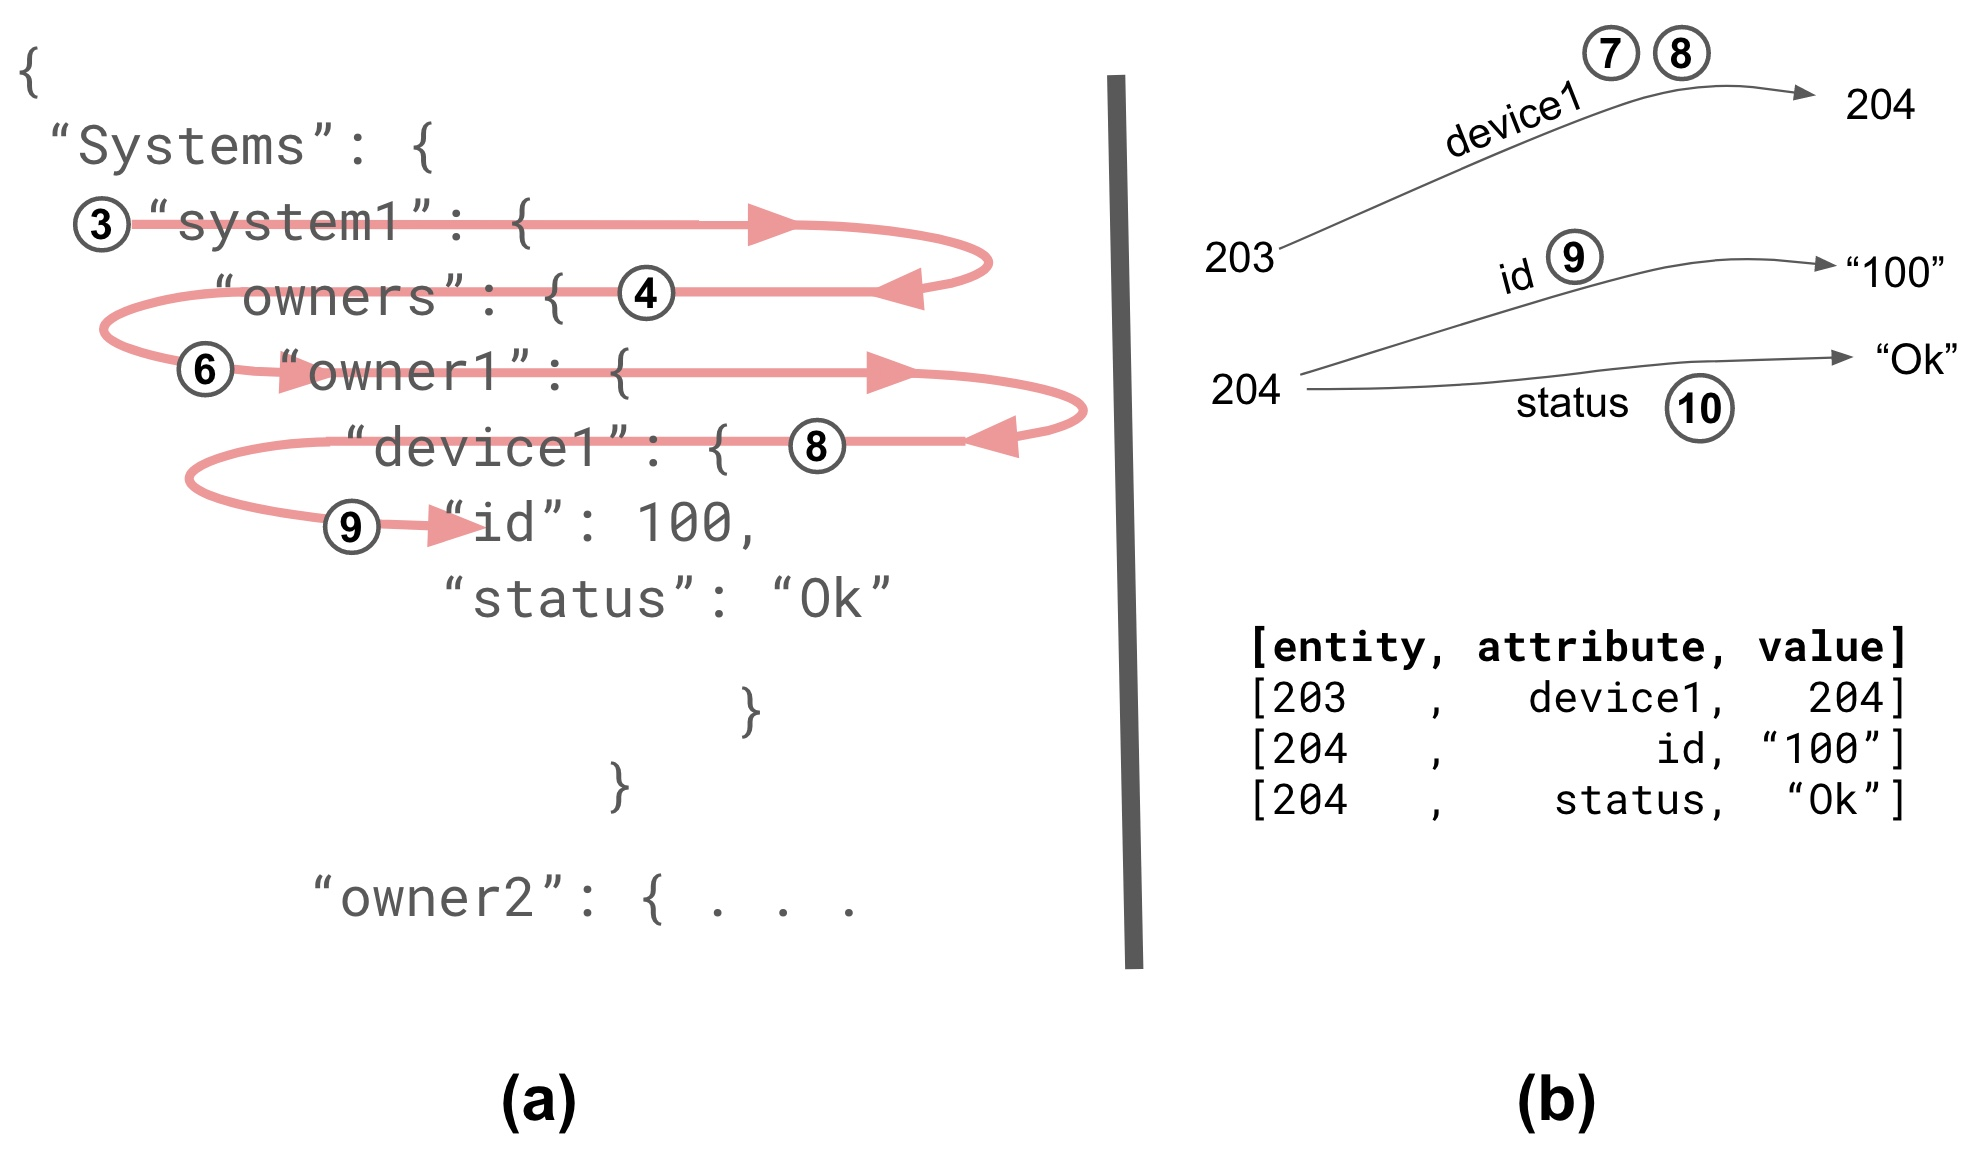
\includegraphics[scale=0.15]{hairpin-two-part.jpg}
  \centering
\end{figure}  \vspace{-1em}

A Datalog database can be viewed as several index tables about the triples (such as those depicted in Figure~\ref{fig:hairpin} (b).)
One such index table will index primarily by entity, another primarily by attribute, etc.
Some of Lines 2--10 in Figure~\ref{code:restruct}, for example, Line 2, \stt{[?s ?systemName ?x]}, have the form of these triples, where respectively \stt{?s}, \stt{?systemName} and \stt{?x} match an entity, attribute, and value.
Line 4, \stt{[?x :owners ?y]}, is similar but the attribute position is occupied by \stt{:owners}.
This triple will match any fact that has the string \stt{"owners"} in its attribute position.
There are two such facts in the data depicted in Figure~\ref{data:restruct}, one on Line 2, and one on Line 6.
In both cases the value position is occupied by another entity reference.
Figure~\ref{fig:hairpin}(b) similarly depicts a triple whose value position references another entity, \stt{[203, device1, 204]}.

Lines 3, 6 and 8 of the query do not use the 3-place triple pattern; they consist of a single JSONata expression wrapped in parentheses.
The expression should be a Boolean (should return true or false).
 Note that the expression uses variable bindings (e.g \stt{?systemName}, \stt{?ownerName}, and \stt{?deviceName}) used in triples of the query.
 \stt{/system\textbackslash d/} is a JavaScript regular expression matching a string containing \stt{"system"} followed by a single digit (the \stt{\textbackslash d} part).
The following paragraph provides a line-by-line summary of how the query in Lines 2--10 works.

\begin{description}
\item[Line 2 \stt{[?s ?systemName ?x]}:] All positions of this triple pattern are occupied by variables, so by itself it would match every triple in the database.
\item[Line 3 \stt{[(\$match(?systemName, /system\textbackslash d/))]}:] This uses the query variable \stt{?systemName} bound to the entity position on Line 2.
  Therefore, between this pattern and the one in Line2, the only triples matching both of these patterns have ``system1'' or ``system2'' in the attribute position. (See the data to verify this.)
  \stt{?s} and \stt{?x} from Line 2 are thus bound to the entity and value positions of triples having either ``system1'' or ``system2'' in their attribute positions.
\item[Line 4 \stt{[?x :owners ?y]}:] Here we see \stt{?x}, which was introduced in Line 2, reused in the entity position.
  We know that \stt{?x} is bound to an entity by looking at the data.
  (See Line 2 in the data for example, \stt{ ``owners'': \{\ldots}. The ``\stt{: \{}'' means the thing keyed by ``owners'' here is a JSON object (an ``entity'' in the database).
  This triple pattern ensures that \stt{?x} refers to entities for \DIFdelbegin \DIFdel{with the }\DIFdelend \DIFaddbegin \DIFadd{which }\DIFaddend "owners" occupies the attribute position.
\item[Line 5 \stt{[?y ?ownerName ?z]}:]  Like Line 2, this is used to introduce \DIFdelbegin \DIFdel{an }\DIFdelend \DIFaddbegin \DIFadd{a }\DIFaddend new variable, \stt{?ownerName} in this case, which will be used in the a \stt{\$match} predicate similar to Line 3.
  One difference here, however, is that the value of \stt{?y} is constrained by the triple pattern on Line 4.
\item[Line 6 \stt{[(\$match(?ownerName, /owner\textbackslash d/))]}:] This serves a similar purpose Line 3, but for owner keys.
\item[Line 7 \stt{[?z ?deviceName ?d]}:] This is like Lines 1 and 5, introducing a new variable for use in the \stt{\$match}.
  Like Line 5, the value of the variable in entity position is constrained by another pattern.
\item[Line 8 \stt{[(\$match(?deviceName, /device\textbackslash d/))]}:] This is similar in purpose to the other two uses of \stt{\$match}.
\item[Line 9 \stt{[?d :id ?id]}:] Here we are finally ready to pick up some user data, the value of a device's ``id'' attribute.
\item[Line 10 \stt{[?d :status ?id]}:] Like Line 9, but to pick up the value of a device's ``status'' attribute.
\end{description}

% Discuss use of key() and vector syntax to create more conventional output.
It was suggested earlier that the encoding of the source data \DIFdelbegin \DIFdel{was }\DIFdelend \DIFaddbegin \DIFadd{in Figure\ref{data:restruct} is }\DIFaddend a bit unusual.
\DIFdelbegin \DIFdel{For example}\DIFdelend \DIFaddbegin \DIFadd{Specifically}\DIFaddend , object key values such as \stt{owner1}, \stt{system1} and \stt{device1} are being used \DIFdelbegin \DIFdel{, apparently, }\DIFdelend both to indicate a unique entity \DIFaddbegin \DIFadd{type (i.e.\~respectively owners, systems, and devices) }\DIFaddend and to identify %DIF < -----the kind of entity being described, presumably an owner, system and device respectively.
\DIFaddbegin \DIFadd{specific instances of those types.
This is bad practice.
Imagine how hard it would be to understand what is going on were the identifiers in Figure\ref{data:restruct} replaced with arbitrary strings such as UUIDs.
}\DIFaddend We might seek target data that explicitly declares the type and identifier separated, for example using attributes \stt{type} and \stt{id} respectively.
The target data sought, for example, might be as depicted in Figure~\ref{data:slack-with-keys}.

\begin{figure}[H]
  \caption{An alternative organization of the target data from the example.}
 \label{data:slack-with-keys}
\begin{lstlisting}[language=JavaScript,basicstyle=\ttfamily\scriptsize,numberstyle=\scriptsize]
[{"type"   : "OWNER",
  "id"     : "owner1",
  "systems": [{"type"   : "SYSTEM",
               "id"     : "system1",
               "devices": [{"type"   : "DEVICE",
                            "id"     : "100",
                            "status" : "Ok"},
                           {"type"   : "DEVICE",
                             "id"    : "200",
                             "status": "Ok"}]},
              {"type"   : "SYSTEM",
               "id"     : "system2",
               "devices": [{"type"   : "DEVICE",
                            "id"     : "500",
                            "status" : "Ok"},
                           {"type"   : "DEVICE",
                             "id"    : "600",
                             "status": "Ok"}]}]},
 {"type"   : "OWNER",
  "id"     : "owner2",
  "systems": [{"type"   : "SYSTEM",
               "id"     : "system1",
               "devices": [{"type"   : "DEVICE",
                            "id"     : "300",
                            "status" : "Ok"},
                           {"type"   : "DEVICE",
                             "id"    : "400",
                             "status": "Ok"}]},
              {"type"   : "SYSTEM",
               "id"     : "system2",
               "devices": [{"type"   : "DEVICE",
                            "id"     : "700",
                            "status" : "Ok"},
                           {"type"   : "DEVICE",
                             "id"    : "800",
                             "status": "Ok"}]}]}]
\end{lstlisting}
\end{figure}  \vspace{-2em}

As the figure depicts, the output is more verbose. % , and only in Hollywood do the colons line up in the columns like that
A guess at an \stt{express} structure to produce this output is as follows.
\begin{figure}[H]
  \caption{Draft express structure for target data as depicted in Figure~\ref{data:slack-with-keys}}
 \label{code:slack-possible-express}
\begin{lstlisting}[language=JavaScript,basicstyle=\ttfamily\scriptsize,numberstyle=\scriptsize]
$ex1 := express{{'owners' : {'type'   : 'OWNER',
                             'id'     : ?ownerName,
                             'systems': [{'type'   : 'SYSTEM',
                                          'id'     : ?systemName,
                                          'devices': [{'type'  : 'DEVICE',
                                                       'id'    : ?deviceName,
                                                       'status': ?status}]}]}}
               }
\end{lstlisting}
\end{figure}  \vspace{-3em}

If we were to map over that \stt{express} body, that is \stt{\$map(\$bsets,\$ex1)}, the result would be \DIFdelbegin \DIFdel{(logically correct , of course but ) }\DIFdelend \DIFaddbegin \DIFadd{logically correct but }\DIFaddend even more verbose and %DIF < -----also repetitive because there will be one full structure like the \stt{express} body for each of the 8 binding sets.
\DIFaddbegin \DIFadd{also repetitive because there will be one full structure like the \stt{express} body for each of the 8 binding sets.
}\DIFaddend A better alternative might be to \stt{\$reduce} over the \stt{express}, that is, \stt{\$reduce(\$bsets,\$ex1)}\DIFdelbegin \DIFdel{;
}\DIFdelend \DIFaddbegin \DIFadd{. 
}\DIFaddend \stt{\$reduce} can have the effect of ``summarizing'' data, in this case by squeezing out the repetition.
However, there is a problem with reducing over the \stt{express} body as written;
it would produce the following:

\begin{figure}[H]
  \caption{Reducing over the \stt{express} body here results in iteratively overwriting data; the result is
    the same as applying \stt{express} body to just the last binding object. \DIFaddbeginFL \DIFaddFL{Data is lost!}\DIFaddendFL }
 \label{code:slack-result-wo-keys}
\begin{lstlisting}[language=JavaScript,basicstyle=\ttfamily\scriptsize,numberstyle=\scriptsize]
{"type"    : "OWNER",
 "id"      : "owner1",
 "systems" : {"type"    : "SYSTEM",
              "id"      : "system1",
              "devices" : {"type"   : "DEVICE",
                           "id"     : "device2",
                           "status" : "Ok"}}}

   /* This result indicates that the last binding object processed was the following */
   {?ownerName : "owner1", ?systemName : "system1", ?deviceName : "device2", ?status : "Ok", ?id : 200}
\end{lstlisting}
\end{figure}  \vspace{-3em}

What happened to the rest of the data?
Why were data not lost similarly when we reduced over the \stt{express} body on Lines 14--20 of Figure~\ref{code:restruct}?
The answer is that the \stt{express} body of Figure~\ref{code:restruct} uses unique values for the object keys.
The effect of reducing over the \stt{express} body in that example is to ``drop in'' new pathways for each binding object.
Specifically, if we consider the Lines 13--21 of Figure~\ref{data:restruct}, the result of applying the \stt{express} body on Lines 14--20 of %-----Figure~\ref{code:restruct} to the key values in each corresponding binding object, it is apparent that:

\begin{itemize}
\item the Line 14 object was created by the keys \stt{"owners"}, \stt{"owners1"}, \stt{"system1"}, \stt{"device1"},
\item the Line 15 object was created by the keys \stt{"owners"}, \stt{"owners1"}, \stt{"system1"}, \stt{"device2"},
\item the Line 16 object was created by the keys \stt{"owners"}, \stt{"owners1"}, \stt{"system2"}, \stt{"device5"}, and
\item et cetera, to Line 21, created by the keys \stt{"owners"}, \stt{"owners2"}, \stt{"system2"}, \stt{"device8"}.
\end{itemize}

There are three solutions to the problem just highlighted:
(1) use unique keys to ``drop in'' new pathways like in the original example,
(2) use \stt{\$map} instead of \stt{\$reduce}, which entails accepting the fact that the result will be verbose with lots of repetition, or
(3) wrap keys in the \stt{key} construct as described below.

\subsubsection{The \stt{key} construct of \stt{express}}

We'll continue with the running example.
In order to prevent the overwriting that was depicted in Figure~\ref{code:slack-result-wo-keys} we will
adapt the code from Figure~\ref{code:slack-possible-express} by adding the \stt{key} construct as shown.

\begin{figure}[H]
  \caption{The express structure from Figure~\ref{code:slack-possible-express} revised to identify keys}
 \label{code:slack-express-with-keys}
\begin{lstlisting}[language=JavaScript,basicstyle=\ttfamily\scriptsize,numberstyle=\scriptsize]
$ex1 := express{{'owners' : {'type'    : 'OWNER',
                              'id'     : key(?ownerName),
                              'systems': [{'type'   : 'SYSTEM',
                                           'id'     : key(?systemName),
                                           'devices': [{'type'  : 'DEVICE',
                                                        'id'    : key(?deviceName),
                                                        'status': ?status}]}]
                            }
                  }
                 }
\end{lstlisting}
\end{figure}  \vspace{-2em}

Here we modified Lines 2, 4, and 6 of Figure~\ref{code:slack-possible-express}, wrapping the binding variables
\stt{?ownerName}, \stt{?systemName}, and \stt{?deviceName} in the \stt{key} construct.
The \stt{key} construct declares identity conditions for the corresponding objects.
With knowledge of identity conditions, reduce processing on the \stt{express} body can distinguish between inserting a new object (one where the key hasn't yet been seen) and updating (or mistakenly overwriting) the existing object.
Thus, the entire source data can be pushed into a single object structured as depicted in the figure.
Incidentally, note that Lines 3 and 5 use square brackets to signify that there are possibly multiple systems and devices respectively
in the target form.

% Right here you might want to show the previous example with namespaced keys and talk about
% how that reduces the cognitive load and dovetails with serialization to namespaced XML.

\subsection{Summary thoughts on \stt{query} and \stt{express}}

\stt{query} and \stt{express} are two principal constructs of the RADmapper language that together provide powerful, flexible, means to restructure data.
They enable mapping from multiple sources, in-place updating, and effective methods of abstraction and composition such as templating and higher-order functions.
It may look like a lot to learn, and in fact there is more to the language yet to be discussed.
That notwithstanding, we believe that many tasks can be programmed with RADmapper more easily than with pure JSONata.
For example, consider  the running example of restructuring we discussed above.
The pure JSONata solution uses lots of syntax and juggling operations (see Figure~\ref{code:jsonata-sTPDRs}) to do something that is conceptually very simple.
The RADmapper solution, on the other hand, reflects those simple observations: with \stt{query} you pull out threads of data that conceptually hang together;
with \stt{express} you either \stt{\$map} or \stt{\$reduce} the individual threads into a result structure.
Separating the collection of source information from the expression of target information makes the task easier to perform.
Further, even these two mostly-independent steps can be approached in smaller sub-steps.
For example, one could start with a \stt{query} that binds just one or two query variables along a path.
When it is clear that that works (verified in the RADmapper exerciser, for example) one could progressively add more path steps until the complete, coherent thread of domain relationships is captured.

Likewise, you can create binding sets by hand and approach programming the \stt{express} structure in small steps.
You can evaluate \stt{express} with a single binding object to see the result, combine binding objects (even from calls to different \stt{query} definitions) and experiment with \stt{\$reduce}-ing on the \stt{express}.

%The motivation for RADmapper, however, is more encompassing than what discussion thus far might suggest.
%Though you can use RADmapper's web-based exerciser to define and validate mappings,
%and you can include RADmapper in Java and JavaScript programs \footnote{RADmapper is available for use in Java and JavaScript programs as a \stt{.jar} file and NPM library respectively. A Docker version of the exerciser is available [URL] and hosted at [URL].} a principal goal of RADmapper is to support \textit{interoperable} mapping. The next section discusses interoperability; you do not need to read it if your primary goal is to learn how to use RADmapper in Java or JavaScript software.

\section{\DIFdelbegin \DIFdel{Exchanging }\DIFdelend \DIFaddbegin \DIFadd{Communicating }\DIFaddend Mapping Requirements \DIFaddbegin \DIFadd{to Others}\DIFaddend , \stt{\$toAST}}
\label{sec:toAST}

RADmapper seeks to describe mapping requirements in ways that are useful to the various stakeholder and tools used in integration efforts.
Describing mapping requirements is but one of the tasks of an integration effort.\DIFdelbegin \DIFdel{By ``integration effort'' we mean work spent to make separate things work jointly towards some goal.
}\DIFdelend \DIFaddbegin \footnote{\DIFadd{By ``integration effort'' we mean work spent to make separate things work jointly towards a shared goal.}}
\DIFaddend The goals of integration efforts \DIFdelbegin \DIFdel{are various }\DIFdelend \DIFaddbegin \DIFadd{vary, }\DIFaddend including, for example, automating the regular purchase of items under a contract, or implementing new sensing capability in automated production.
The stakeholders in integration efforts typically include at least
(1) domain experts, the people who can describe what the entities (e.g.\DIFaddbegin \DIFadd{~}\DIFaddend business entities, machines) need to do in the joint work,
(2) back-end system administrators, that manage the databases involved in the kinds of transactions of interest, and
(3) API programmers, who implement the code that achieves the goals of the integration.
In small enterprises, of course, many of these roles are played by a single person.

The RADmapper language presented in Section~\ref{sec:quick-start} \DIFdelbegin \DIFdel{, }\DIFdelend \DIFaddbegin \DIFadd{is }\DIFaddend a human-oriented domain-specific language (DSL).
The exchange format\DIFaddbegin \DIFadd{, however, }\DIFaddend should not be a human-oriented DSL because such a requirement would force users of RADmapper to parse the \DIFdelbegin \DIFdel{language}\DIFdelend \DIFaddbegin \DIFadd{syntax}\DIFaddend .
Because the DSL language is mostly declarative and functional, however, the syntax avoids procedural constructs like loops and indexing.
Consequently, it is reasonable to express RADmapper DSL as an easily navigable tree structure;
the \textit{abstract syntax tree} (AST) of the language provides such trees.
We implemented this idea as a RADmapper DSL function called \stt{\$toAST}, which takes a string of any valid RADmapper DSL expression, and returns a tree parsable as \DIFdelbegin \DIFdel{Javascript }\DIFdelend \DIFaddbegin \DIFadd{JavaScript }\DIFaddend Object Notation (JSON).
Figure~\ref{fig:mapping-src2tar-toAST} below depicts the result of applying to the RADmapper code of Figure~\ref{fig:mapping-src2tar} taken as a string.

\begin{figure}[H]
  \caption{Canonical serialization of the mapping function from Figure~\ref{fig:mapping-src2tar} as JSON.
    Alternatives of the canonical exchange form are easily implemented as other mapping tasks.}
 \label{fig:mapping-src2tar-toAST}
\DIFmodbegin
\begin{lstlisting}[language=JavaScript,basicstyle=\ttfamily\scriptsize,numberstyle=\scriptsize,alsolanguage=DIFcode]
%DIF < {"FnDef" : {"Params" : ["$d"]}, //  $d is a source data structure
%DIF > {"FnDef" : {"Params" : ["$d"]}, //  $d is a source data structure.
 "Body" :
 {"Object" :
  {"Invoice" :
   {"Object" :
    {"DataArea" :
     {"Object" :
      {"ApplicationArea" :
       {"Object" :
        {"CreationDateTime" :
         {"BinaryExpression" : ["$d","get","Invoice","get","ApplicationArea","get","CreationDateTime"]}}},
       "Invoice" :
       {"Object" :
        {"InvoiceLine" :
         {"Object" :
          {"BuyerParty" :
           {"Object" :
            {"Location" :
             {"Object" : {"Address" :
                          {"Object" : {"BuildingNumber" :
                                       {"rm.$llmExtract" :
                                        {"args" : [{"BinaryExpression" :
                                                    ["$d","get","Invoice","get","DataArea","get","Invoice",
                                                     "get","InvoiceLine","get","BuyerParty","get","Location",
                                                     "get","Address","get","AddressLine"]},
                                                   "BuildingNumber"]}},
                                       "CityName" :
                                       {"rm.$llmExtract" :
                                        {"args" : [{"BinaryExpression" :
                                                    ["$d","get","Invoice","get","DataArea","get","Invoice",
                                                     "get","InvoiceLine","get","BuyerParty","get","Location",
                                                     "get","Address","get","AddressLine"]},
                                                   "CityName"]}},
                                       "PostalCode" :
                                       {"rm.$llmExtract" :
                                        {"args" : [{"BinaryExpression" :
                                                    ["$d","get","Invoice","get","DataArea","get","Invoice",
                                                     "get","InvoiceLine","get","BuyerParty","get","Location",
                                                     "get","Address","get","AddressLine"]},
                                                   "PostalCode"]}},
                                       "StreetName" :
                                       {"rm.$llmExtract" :
                                        {"args" : [{"BinaryExpression" :
                                                    ["$d","get","Invoice","get","DataArea","get","Invoice",
                                                     "get","InvoiceLine","get","BuyerParty","get","Location",
                                                     "get","Address","get","AddressLine"]},
                                                   "StreetName"]}}}}}},
             "TaxIDSet" : {"Object" : {"ID" : {"BinaryExpression" : ["$d","get","Invoice","get","DataArea",
                                                                     "get","Invoice","get","InvoiceLine",
                                                                     "get","BuyerParty",
                                                                     "get","TaxIDSet","get","ID"]}}}}},
           "Item" : {"Object" : {"ManufacturingParty" :
                                 {"Object" : {"Name" : {"BinaryExpression" : ["$d","get","Invoice",
                                                                              "get","DataArea",
                                                                              "get","Invoice","get","InvoiceLine",
                                                                              "get","Item",
                                                                              "get","ManufacturingParty",
                                                                              "get","Name"]}}}}},
           "PurchaseOrderReference" : {"Object" : {"ID" : {"BinaryExpression" :
                                                           ["$d","get","Invoice","get","DataArea","get","Invoice",
                                                            "get","InvoiceHeader","get","PurchaseOrderReference",
                                                            "get","ID"]}}}}},
         "Process" : {"BinaryExpression" : ["$d","get","Invoice","get","DataArea","get","Process"]}}}}}}}}}}
\end{lstlisting}
\DIFmodend
\end{figure}  \vspace{-3em}

 \appendix
 \pagebreak

 \renewcommand{\thesection}{Appendix \Alph{section}} % https://tex.stackexchange.com/questions/82235/adding-text-to-the-section-numbering

\section{RDF and OWL Mapping Example}

The following example illustrates mapping of a network of Web Ontology Language (OWL) data to a relational form.
The source OWL data used is simplified from actual OWL data to allow easier discussion.
The data consists of objects of two types, one is OWL classes; these have the value  \stt{owl/Class} in their \stt{rdf/type} attribute.
The other is OWL properties (\stt{owl/ObjectProperty}).
The simplifications include using single values for \stt{rdfs/domain}, \stt{rdfs/range}, and \stt{rdfs/subClassOf}.
An OWL class and property is depicted in Figure~\ref{code:endurant}.

\begin{figure}[H]
  \caption{An object (owl/Class) and a relation (owl/ObjectProperty) in the source population.
    These are somewhat simplified from realistic OWL data.}
  \label{code:endurant}
\DIFmodbegin
\begin{lstlisting}[numberstyle=\scriptsize,basicstyle=\ttfamily\scriptsize,numbers=left,stepnumber=1,breaklines=true,alsolanguage=DIFcode]
{'resource/iri'       : 'dol/endurant',
 'resource/name'      : 'endurant',
 'resource/namespace' : 'dol',
 'rdf/type'           : 'owl/Class',
 'rdfs/comment'       : ['The main characteristic of endurants is...'],
%DIF <  'rdfs/subClassOf     : :dol/spatio-temporal-particular,
%DIF >  'rdfs/subClassOf     : 'dol/spatio-temporal-particular',
 'owl/disjointWith'   : ['dol/abstract', 'dol/quality', 'dol/perdurant']}

{'resource/iri'       : 'dol/participant',
 'resource/name'      : 'participant',
 'resource/namespace' : 'dol',
 'rdf/type'           : 'owl/ObjectProperty',
 'rdfs/comment'       : ['The immediate relation holding between endurants and perdurants...'],
 'owl/inverseOf'      : 'dol/participant-in',
 'rdfs/domain'        : 'dol/perdurant',
 'rdfs/range'         : 'dol/endurant'}
\end{lstlisting}
\DIFmodend
\end{figure} \vspace{-3em}

The target data we'll be creating consists of three kinds of things: schema, tables, and columns.
Even with this simple data, there are a few options for designing the relational schema.
The following are design choices that define the form of the mapping target:
\begin{enumerate}
\item Both \stt{owl/Class} and \stt{owl/ObjectProperty} can have \stt{rdfs/comment} and the relationship is one-to-many.
  A single table with keys consisting of the resource IRI and comment text will suffice.

\item \stt{rdf/type} is one-to-one with the class. Though the possible values are limited to just a few such as \stt{owl/Class} and
  \stt{owl/ObjectProperty}, we will represent it with a string naming the type.

\item \stt{resource/name} and \stt{resource/namespace} are also one-to-one and are just the two parts of \stt{resource/iri} and could be computed, but we will store these in the class table too.

\item We will assume \stt{rdfs/domain},  \stt{rdfs/range}, and \stt{rdfs/subClassOf} are single-valued. Typically they are not in a real OWL ontology.

\item We will assume that we want to support storage of individuals of the types defined by OWL classes.
  Though our approach here is not at all reflective of description logic, where class subsumption is the primary kind of inference,
  mapping will produce a two-column table where one column is the individual's IRI and the other is the foreign key of a class to which it belongs.

\item We will assume that all relations are conceptually binary.
  Thus storing individuals means that for each \stt{owl/ObjectProperty} mapping will produce a two-column table to represent both a relation and its inverse (``inverse pairs'') where an inverse is defined.
  Such a table works in both directions (the relation and its inverse), so we will have to prevent creating a table for one member of each inverse pair.

\end{enumerate}

% To keep things simple, we'll omit some otherwise useful considerations like identifying what columns define keys;
%[This belongs elsewhere]: A table keyed by a class \stt{resource/iri} will be defined to store the \stt{resource/name} and \stt{resource/namespace}.
%
With the above considerations in mind, it becomes apparent that some of the work involves nothing more than storing class and property metadata into tables we can define ahead of time.
The \stt{owl/ObjectProperty} definitions, however, entails one new table for each relation (or relation pair if an inverse is defined).
The rows of these tables would be populated by instances of the classes specified by \stt{rdfs/domain} and \stt{rdfs/range}.
This information is not in the ontology, but Figure~\ref{code:static-ddl} depicts the static tables in typical relational DDL.
These are populated by the ontology \stt{owl/Class} content of the
Figure~\ref{code:dynamic-ddl-dml} depicts tables that would be created.

% ToDo: Get listinglst for SQL
\begin{figure}[H]
  \caption{Static DDL for storing class and object relation metadata.
  The mapping will generate information equivalent to DML to populate this from the source data.}
  \label{code:static-ddl}
\begin{lstlisting}[numberstyle=\scriptsize,basicstyle=\ttfamily\scriptsize,numbers=left,stepnumber=1,breaklines=true]
  CREATE SCHEMA typicalOWL;

  CREATE TABLE ObjectDefinition
    (resourceIRI       VARCHAR(300) primary key,
     resourceLabel     VARCHAR(300) not null,
     resourceNamespace VARCHAR(300) not null);

  CREATE TABLE ClassDefinition
    (resourceIRI VARCHAR(300) primary key,
     subClassOf  VARCHAR(300) references ClassDefinition);

  CREATE TABLE ObjectClass
    (resourceIRI VARCHAR(300) primary key,
     class       VARCHAR(300) references ClassDefinition);

  CREATE TABLE DisjointClass
    (disjointID  INT primary key,
     disjoint1   VARCHAR(300) not null references ObjectDefinition,
     disjoint2   VARCHAR(300) not null references ObjectDefinition);

  CREATE TABLE ResourceComment
    (commentID    INT primary key,
     resourceIRI  VARCHAR(300) not null references ObjectDefinition,
     commentText  VARCHAR(900) not null);

  CREATE TABLE PropertyDefinition
    (resourceIRI    VARCHAR(300) primary key,
     relationDomain VARCHAR(300) references ObjectDefinition,
     relationRange  VARCHAR(300) references ObjectDefinition);
\end{lstlisting}
\end{figure} \vspace{-3em}

Figure~\ref{code:dynamic-ddl-dml} depicts the result of mapping data from Figure~\ref{code:endurant} using a mapping
specification that will be described below.

\begin{figure}[H]
  \caption{Result of mapping the data depicted in Figure~\ref{code:endurant}.
    This specifies content equivalent to
    (1) DML to capture metadata for owl/Class and owl/ObjectProperty objects in the static tables defined above, and
    (2) DDL to create tables for owl/ObjectProperty objects.}
  \label{code:dynamic-ddl-dml}
\begin{lstlisting}[language=JavaScript,numberstyle=\scriptsize,basicstyle=\ttfamily\scriptsize,numbers=left,stepnumber=1,breaklines=true]
  {'instance-of'  : 'insert-row',
   'table'        : 'ObjectDefinition',
   'content'      : [{'resourceIRI'       : 'dol/endurant'},
                     {'resourceLabel'     : 'endurant'},
                     {'resourceNamespace' : 'dol'}]}

  {'instance-of'  : 'insert-row',
   'table'        : 'ClassDefinition',
   'content'      : [{'resourceIRI'    : 'dol/endurant'},
                     {'subClassOf'     : 'dol/spatio-temporal-particular'}]}

  {'instance-of'  : 'insert-row',
   'table'        : 'DisjointClass',
   'content'      : [{'disjointID'   ; 1},
                     {'disjoint1'    : 'dol/endurant'},
                     {'disjoint2'    : 'dol/abstract'}]} /* ... (Two more disjoints elided.) */

  {'instance-of'  : 'insert-row',
   'table'        : 'ResourceComment',
   'content'      : [{'commentID'   : 1},
                     {'resourceIRI' : 'dol/endurant'},
                     {'commentText' : 'The main characteristic of endurants is...'}]}

  /* Similar content for the ObjectPropery dol/participant is elided. */

  {'instance-of'  : 'insert-row',
   'table'        : 'PropertyDefinition',
   'content'      : [{'resourceIRI'    : 'dol/participant'},
                     {'relationDomain' : 'dol/perdurant'},
                     {'relationRange'  : 'dol/endurant'}]}

  /* The DDL for the participant table: */

  {'instance-of' : 'create-table',
   'table'       : 'DOLparticipant',
   'columns'     : [{'colName' : 'propertyID',
                     'dtype'   : {'type' : 'varchar', 'size' : 300, 'key' : 'primary'}},
                    {'colName' : 'role1',
                     'dtype'   : {'type' : 'varchar', 'size' : 300, 'ref' : 'ObjectDefinition'}},
                    {'colName' : 'role2',
                     'dtype'   : {'type' : 'varchar', 'size' : 300, 'ref' : 'ObjectDefinition'}}]}
\end{lstlisting}
\end{figure} \vspace{-3em}

%Schema for the target data (the table definitions, etc.) is depicted in Figure ~\ref{code:example-schema-1}.
%The object types define attributes (\stt{db/attrs}) and keys (\stt{db/key}).
%Each attribute has a type (\stt{db/type}) and a cardinality (\stt{db/cardinality}.
%The \stt{db/type} can be any primitive type defined (e.g. strings, numbers, UUID, etc.) or \stt{object}, meaning that
%the attribute is populated by either references to other objects (foreign keys) or objects in-lined in the structure, the choice depending on the value of \stt{db/in-line?}.

%The top-level entries in this schema are identified
%by the strings ``schema'', ``table'', and ``column'' which have no particular significance but might be used in
%error reporting (or we'll get rid of them).

% ToDo: Did I decide to move :db/key ??? If so, do I really need the nested structure?
% ToDo: Do I really want table/schema, or do I want schema/tables?
% \begin{figure}[H]
%   \caption{A schema for the target data}
%   \label{code:example-schema-1}
% \begin{lstlisting}[numberstyle=\scriptsize,basicstyle=\ttfamily\scriptsize,numbers=left,stepnumber=1,breaklines=true]
%   [{'schema' : {'db/attrs'  : [{'schema/name'   : {'db/type' : 'string', 'db/cardinality' : 'one'}}],
%                 'db/key'    : ['schema/name']}}
%
%    {'table'  : {'db/attrs'  : [{'table/name'    : {'db/type' : 'string', 'db/cardinality' : 'one' },
%                                 'table/schema'  : {'db/type' : 'object', 'db/cardinality' : 'one',
%                                                    'db/in-line?' : true},
%                                 'table/columns' : {'db/type' : 'object', 'db/cardinality' : 'many'}}],
%                 'db/key'    : ['table/schema', 'table/name']}}
%
%    {'column' : {'db/attrs'  : [{'column/name'   : {'db/type' : 'string', 'db/cardinality' : 'one'}},
%                                {'column/type'   : {'db/type' : 'string', 'db/cardinality' : 'one'}},
%                                {'column/table'  : {'db/type' : 'object', 'db/cardinality' : 'one'}}],
%                 'db/key'    : ['column/table', 'column/name']}}]
% \end{lstlisting}
% \end{figure}

% The \stt{db/cardinality} of all the attributes in ``one'' except in the case of \stt{table/columns} which is ``many''.
% (See Line 7 of the figure.)
% Cardinality of one means that actions on this attribute of an object necessarily either creates the triple or updates it.
% There will never be two triples about this attribute in the target population where the first two elements of the triple are identical.
% Cardinality of many means that that there could be multiple triples for the attribute.
% Keep in mind that the elements of a triple are always atomic.
% To represent $n$ values there are $n$ triples having different values for the third element of the triple.
% Also, the underlying datalog tool preserves the order of elements in arrays.
%
% Line 7 in the figure demonstrates the use of the optional, \stt{db/in-line?} schema feature.
% On Line7 \stt{db/in-line?} is set to true (the default is false).
% \stt{db/in-line?} true directs the mapper to create structures rather than references.
% Relation technology provides nothing quite like in-lining, but we demonstrate its use in the example below nonetheless.
% In the example, schema are described by just their name; entire objects are serialized like this: \stt{\{schema/name ``some schema''\}}.
% It seems reasonable in these circumstances to in-line, much less so in the case of the back-pointer \stt{table/columns}.

Figure~\ref{code:mapping-owl-to-rdbms} depicts the complete specification of a transformation of the source.
\stt{\$transform} is a side-effecting function that takes three arguments, a data context, a binding set, and an express function;
it returns a connection to resulting data.
(Returning the data itself might not be reasonable in the case that it is very large and managed by a database.)
When the binding set argument is a literal call to \stt{query} it is possible for the parser to do syntax checking between
the \stt{query} and \stt{express}.

The \stt{query} produces a binding set for the source data.
The \stt{express} defines how values from each binding object in the binding set are used in the target population.

%DIF <  ToDo: Check out the URL about better listing javascript
%DIF >  ToDo: Check out the URL about better listing JavaScript
% https://mysnippets443.wordpress.com/2015/11/28/latex-insert-javascript-code-with-lstlisting-package/

\begin{figure}[H]
  \caption{Mapping the example OWL to the relational database schema}
  \label{code:mapping-owl-to-rdbms}
\DIFmodbegin
\begin{lstlisting}[language=JavaScript,numberstyle=\scriptsize,basicstyle=\ttfamily\scriptsize,numbers=left,stepnumber=1,breaklines=true,alsolanguage=DIFcode]
  (   $data := $read('data/testing/owl-example.edn');

  $qtype  := query($rdfType, $extraTrips)
               { [?class :rdf/type            $rdfType]
                 [?class :resource/iri        ?class-iri]
                 [?class :resource/namespace  ?class-ns]
                 [?class :resource/name       ?class-name]
                 /* ToDo: $extraTrips */
               };  /* Defines a higher-order function, a template of sorts. */

%DIF <   $etype  := enforce($tableType)
%DIF >   $etype  := express($tableType)
              {  {'instance-of'  : 'insert-row',
                  'table'        : $tableType,
                  'content'      : {'resourceIRI'       : ?class-iri,
                                    'resourceNamespace' : ?class-ns,
                                    'resourceLabel'     : ?class-name}}
%DIF <                            }; /* Likewise, for an enforce template. */
%DIF >                            }; /* Likewise, for an express template. */
                              /* The target tables for objects and relations a very similar. */

  $quClass := $qtype('owl/Class');     /* Use the template, here and the next three assignments. */

  /* This one doesn't just specify a value for $rdfType, but for $extraTrips. */
  $quProp       := $qtype('owl/ObjectProperty'); /* ToDo: ,queryTriples{[?class :rdfs/domain ?domain] [?class :rdfs/range ?range]}); */
  $enClassTable := $etype('ClassDefinition');
  $enPropTable  := $etype('PropertyDefinition');

  /* Run the class query; return a collection of binding objects about classes. */
  $clasBsets := $quClass($data);

  /* We start enforcing with no data, thus the third argument is []. */
  $tar_data := $reduce($clasBsets, $enClassTable, []);

  /* Get the binding set for the ObjectProperties and make similar tables. */
  $propBsets := $quProp($data);

  /* We pass in the target data created so far. */
  $reduce($propBsets, $enPropTable, $tar_data) /* The code block returns the target data. */
)
\end{lstlisting}
\DIFmodend
\end{figure} \vspace{-3em}

% ToDo: This needs work.
The example dataset from DOLCE is fairly large.
Let's suppose it contains 50 classes, each involved in 10 relations.
That suggests a collection of 500 binding objects.
That does not necessarily entail 500 structures like Lines 10 through 14, however.
In contrast to the JSONata-like operations, which maps physical structures to physical structures,
the mapping engine here is mapping between logical structures.
Specifically, a triple represents a fact and the database of triples need only represent a fact once.
It is the knowledge of keys and references provided by the schema that allows the mapping engine to construct physical structure
from the logical relationship defined by the mapping specification.


\bibliography{/home/pdenno/Documents/bibtex/MainCollection}

\end{document}
%%% Local Variables:
%%% mode: latex
%%% TeX-master: "interop-mapping"
%%% End:
